\documentclass[dvipdfmx,13pt,aspectratio=169]{beamer}

\usepackage{animate}
% \usepackage{svg}

\usepackage{adjustbox}      % \begin{adjustbox}
\usepackage[linesnumbered, ruled, vlined]{algorithm2e}    % \begin{algorithm2e}
\usepackage{amsmath}        % \begin{align*}
\usepackage{amssymb}        % \mathbb{A}
\usepackage{amsthm}         % \newtheorem
\usepackage{bm,bbm}         % \bm{A}, \bbm{1}
\usepackage{booktabs}       % \toprule, \midrule, \bottomrule
\usepackage{enumitem}       % \begin{enumerate}[label=(\alph*)]
\usepackage{hyperref}       % \href{URL}{text}
\usepackage{ifthen}         % \ifthenelse
\usepackage{lipsum}         % \lipsum
\usepackage{makecell}       % \makecell{L1\L2}
\usepackage{mathrsfs}       % \mathscr{A}
\usepackage{mathtools}      % \mathrlap
\usepackage{multirow}       % \multirow
\usepackage{optidef}        % \begin{mini*}{x}{f(x)}{}{}
\usepackage{orcidlink}      % \orcidlink
\usepackage{physics}        % \qty, \norm, \abs
\usepackage{subcaption}     % \captionsetup
\usepackage{subfiles}       % \subfile{file}
\usepackage{thm-restate}    % \begin{restatable}{theorem}{thm}
\usepackage{tikz}           % \begin{tikzpicture}
\usepackage{xparse}         % \NewDocumentCommand

\definecolor{cA}{HTML}{0072BD}
\definecolor{cB}{HTML}{EDB120}
\definecolor{cC}{HTML}{77AC30}
\definecolor{cD}{HTML}{D95319}

\newcommand{\red}[1]{\textcolor{red}{#1}}
\newcommand{\blue}[1]{\textcolor{blue}{#1}}
\newcommand{\cyan}[1]{\textcolor{cyan}{#1}}
\newcommand{\gray}[1]{\textcolor{gray}{#1}}
\newcommand{\green}[1]{\textcolor{green}{#1}}
\newcommand{\brown}[1]{\textcolor{brown}{#1}}
\newcommand{\black}[1]{\textcolor{black}{#1}}
\newcommand{\orange}[1]{\textcolor{orange}{#1}}
\newcommand{\purple}[1]{\textcolor{purple}{#1}}
\newcommand{\tccA}[1]{\textcolor{cA}{#1}}
\newcommand{\tccB}[1]{\textcolor{cB}{#1}}
\newcommand{\tccC}[1]{\textcolor{cC}{#1}}
\newcommand{\tccD}[1]{\textcolor{cD}{#1}}
\newcommand{\st}{\text{ s.t. }}
\newcommand{\Img}[1]{\mathrm{Im}\qty(#1)}
\newcommand{\Ker}[1]{\mathrm{Ker}\qty(#1)}
\newcommand{\Supp}[1]{\mathrm{supp}\qty(#1)}
\newcommand{\Rank}[1]{\mathrm{rank}\qty(#1)}
\newcommand{\floor}[1]{\left\lfloor #1 \right\rfloor}
\newcommand{\ceil}[1]{\left\lceil #1 \right\rceil}
% C++ (https://tex.stackexchange.com/questions/4302/prettiest-way-to-typeset-c-cplusplus)
\newcommand{\Cpp}{C\nolinebreak[4]\hspace{-.05em}\raisebox{.4ex}{\relsize{-3}{\textbf{++}}}}
% https://tex.stackexchange.com/questions/28836/typesetting-the-define-equals-symbol
\newcommand{\defeq}{\coloneqq}
\newcommand{\eqdef}{\eqqcolon}
% https://tex.stackexchange.com/questions/5502/how-to-get-a-mid-binary-relation-that-grows
\newcommand{\relmiddle}[1]{\mathrel{}\middle#1\mathrel{}}

% https://tex.stackexchange.com/questions/564216/newcommand-for-each-letter
\ExplSyntaxOn
\NewDocumentCommand{\definealphabet}{mmmm}{
\int_step_inline:nnn{`#3}{`#4}{
\cs_new_protected:cpx{#1 \char_generate:nn{##1}{11}}{
\exp_not:N #2{\char_generate:nn{##1}{11}}}}}
\ExplSyntaxOff

\definealphabet{bb}{\mathbb}{A}{Z}
\definealphabet{rm}{\mathrm}{A}{Z}
\definealphabet{cal}{\mathcal}{A}{Z}
\definealphabet{frak}{\mathfrak}{a}{z}
% \definealphabet{scr}{\mathscr}{A}{Z}
% \definealphabet{frak}{\mathfrak}{A}{Z}

% https://qiita.com/rityo_masu/items/efd44bc8f9229e014237
\allowdisplaybreaks[4]

\usetikzlibrary{
  3d,
  % fit,
  calc,
  math,
  matrix,
  patterns,
  backgrounds,
  arrows.meta,
  shapes.geometric,
  decorations.pathmorphing,
}

% === Beamer Settings ===

% https://uplatexmemo.hatenadiary.jp/entry/2021/01/04/130013
\usepackage{caption}
\captionsetup[figure]{justification=centering}

\usetheme{Boadilla}
\usefonttheme{structurebold}
\useinnertheme{circles}
\setbeamerfont{alerted text}{series=\bfseries}
\setbeamerfont{section in toc}{series=\mdseries}
\setbeamerfont{itemize/enumerate body}{size=\large}
\setbeamertemplate{blocks}[rounded]
\setbeamertemplate{navigation symbols}{}
\setbeamertemplate{footline}[frame number]
\setbeamertemplate{title page}{%
\centering
    \vspace{2.5em}
    {\usebeamerfont{title} \usebeamercolor[fg]{title} \inserttitle \par}
    {\usebeamerfont{subtitle}\usebeamercolor[fg]{subtitle} \insertsubtitle \par}
    \vspace{3.0em}
    \usebeamerfont{author}\insertauthor\par
    \usebeamerfont{institute}\insertinstitute \par
    \vspace{1.5em}
    \usebeamerfont{date}\insertdate\par
    \usebeamercolor[fg]{titlegraphic}\inserttitlegraphic
}

%Beamer Color
\definecolor{blendedblue}{rgb}{0.2,0.2,0.7}
\definecolor{UniBlue}{RGB}{0,150,200} 
\definecolor{UniGreen}{RGB}{0,200,150}
\definecolor{AlertOrange}{RGB}{255,76,0}
\definecolor{AlmostBlack}{RGB}{38,38,38}
\setbeamercolor{normal text}{fg=AlmostBlack}
\setbeamercolor{structure}{fg=UniGreen}
\setbeamercolor{block title}{fg=UniGreen!50!black}
\setbeamercolor{alerted text}{fg=AlertOrange}
\setbeamercolor{itemize item}{fg=black}
\setbeamercolor{itemize subitem}{fg=black}
\setbeamercolor{itemize subsubitem}{fg=black}

\hypersetup{colorlinks=true,linkcolor=UniGreen,citecolor=blue,urlcolor=blue}

\setbeamerfont{section in toc}{size=\LARGE}
\AtBeginSection[]{
    \frame{\tableofcontents[currentsection, hideallsubsections]}
}

% === TITLE ===
\title{\huge{Initial Placement\\for Fruchterman--Reingold Force Model\\with Coordinate Newton Direction}}
\author{\Large{Hiroki Hamaguchi}}
\institute{\large{5th lab}\\\large{Supervisor: Prof. Akiko Takeda}}
\date{2024/12/23}

\newif\ifShowHidden
% \ShowHiddenfalse
\ShowHiddentrue

\begin{document}

\ifShowHidden
  \maketitle
\fi

\ifShowHidden
  \section{Introduction}
\fi

\ifShowHidden
  \begin{frame}{Introduction of Graph Drawing}
    \begin{columns}
      \begin{column}{0.58\columnwidth}
        \large{%
          Graph $G = (V,E)$ (vertices $V$  / edges $E$)\\
          \textbf{Graph Drawing} \normalsize{is an fundamental task.}\\
          \textbf{Force-directed graph drawing} \normalsize{is a popular method.}
        }
        \begin{figure}[htbp]
          \centering
          \begin{minipage}{0.55\columnwidth}
            \centering
            
\includegraphics[width=\columnwidth]{introExample/social.jpg}
            \caption*{
              Social Network Graph
              \gray{\footnotesize{Designed~by~\href{www.freepik.com}{Freepik}}}
            }
          \end{minipage}%
          \begin{minipage}{0.45\columnwidth}
            \centering
            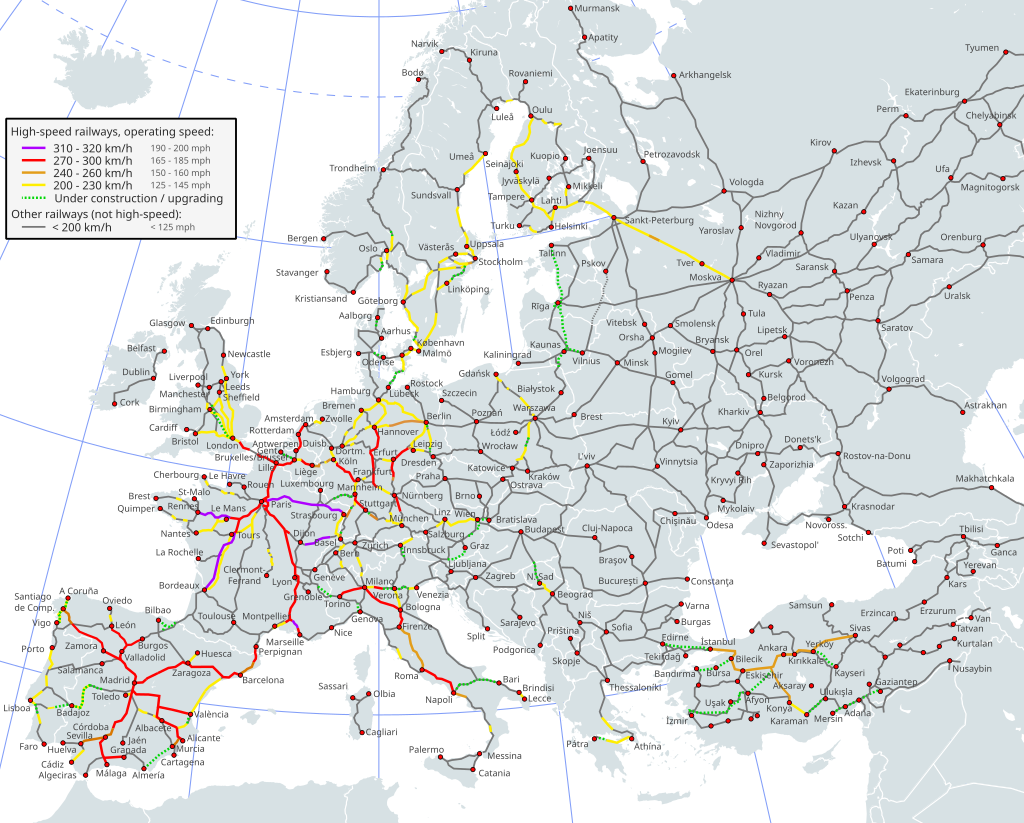
\includegraphics[width=\columnwidth]{introExample/railway.png}
            \caption*{
              Railroad Graph
              \gray{\footnotesize{By~\href{https://commons.wikimedia.org/wiki/File:High_Speed_Railroad_Map_of_Europe.svg}{Bernese~media}, \href{https://creativecommons.org/licenses/by-sa/3.0}{CC~BY-SA~3.0}}}
            }
          \end{minipage}%
        \end{figure}
      \end{column}
      \begin{column}{0.42\columnwidth}
        \centering
        \vspace{-1.5em}
        \begin{figure}[htbp]
          \centering
          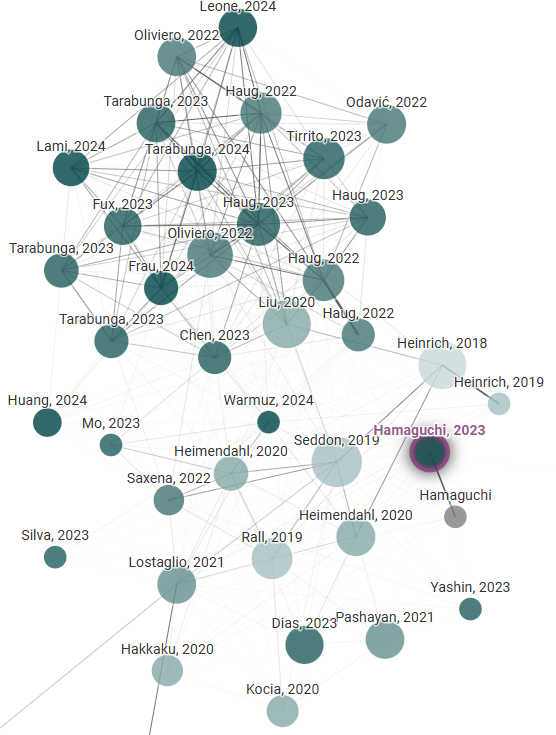
\includegraphics[height=0.77\textheight]{introExample/connectedPapers.png}
          \caption*{
            \gray{\footnotesize{By~\raisebox{-0.4\baselineskip}{
\includegraphics[height=0.07\textheight]{introExample/connectedPapersLogo.png}}
                (\href{https://www.connectedpapers.com/}{Link})}
            }}
        \end{figure}
      \end{column}
    \end{columns}
  \end{frame}
\fi

\ifShowHidden
  \begin{frame}{Graph Drawing by NetworkX}
    \begin{columns}
      \begin{column}{0.62\columnwidth}
        \large{%
          \textbf{Fruchterman--Reingold (FR)} force model is prominent; flexible, intuitive, and simple.\\[1em]
          \textbf{NetworkX} \raisebox{-0.2\baselineskip}{
\includegraphics[width=1.5em]{graphDrawing/networkxLogo.png}}~\cite{hagberg2008exploring} is a popular Python library.\\
          \texttt{nx.draw}: \large{\textbf{FR algorithm}} works with 50 iterations.
        }
        \begin{center}
          \rule{0.8\columnwidth}{0.4pt}
        \end{center}
        \Large{
          \uncover<1->{$\abs{V}=\phantom{0}10$: \phantom{1}0.2 sec / Well Visualized}\\
          \uncover<2->{$\abs{V}=\phantom{0}20$: \phantom{1}0.2 sec / Tangled?}\\
          \uncover<3->{$\abs{V}=500$: \red{11.5} sec / \red{WHAT IS THIS???}}
        }
      \end{column}
      \begin{column}{0.38\columnwidth}
        \begin{figure}[htbp]
          \centering
          \only<1>{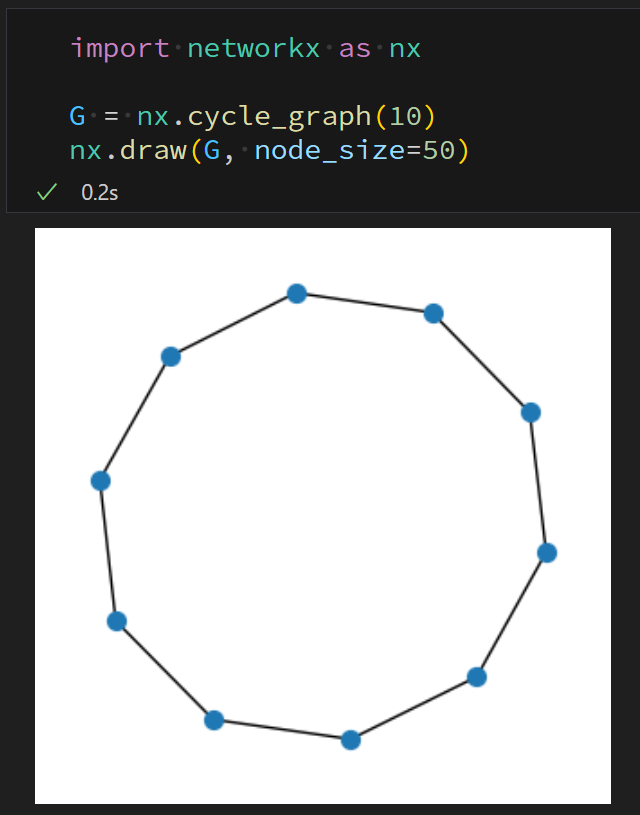
\includegraphics[width=\columnwidth]{vscode/10.png}}%
          \only<2>{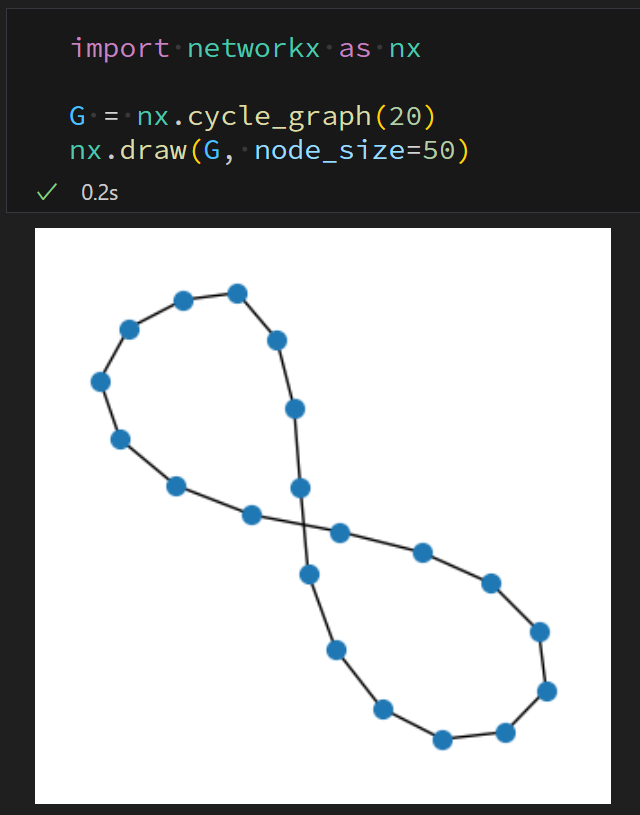
\includegraphics[width=\columnwidth]{vscode/20.png}}%
          \only<3>{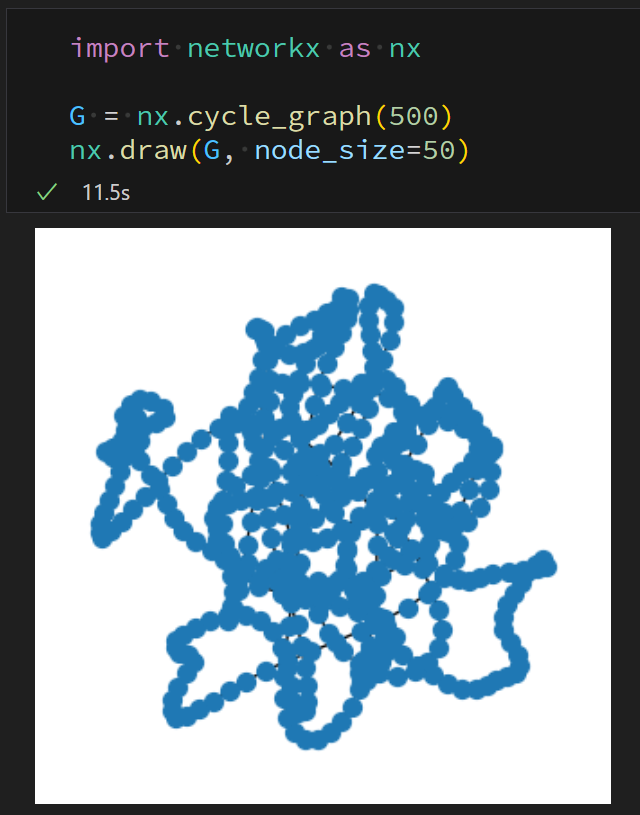
\includegraphics[width=\columnwidth]{vscode/500.png}}%
        \end{figure}
      \end{column}
    \end{columns}
  \end{frame}
\fi

\ifShowHidden
  \begin{frame}{Fruchterman--Reingold Force Model}
    The \textbf{FR force model} uses a force model~\cite{fruchtermanGraphDrawingForcedirected1991} with
    \tccA{\Large{\textbf{a}}}\tccA{ttractive force} and
    \tccD{\Large{\textbf{r}}}\tccD{epulsive force}:
    \begin{equation*}
      \tccA{F_{i,j}^\mathrm{a}(d) \defeq \frac{w_{i,j} d^2}{k}}, \quad \tccD{F^\mathrm{r}(d) \defeq -\frac{k^2}{d}}.
    \end{equation*}
    The \textbf{FR algorithm} seeks an \textbf{equilibrium} of two kind forces:
    \begin{columns}
      \begin{column}{0.5\columnwidth}
        \begin{figure}[h]
          \centering
          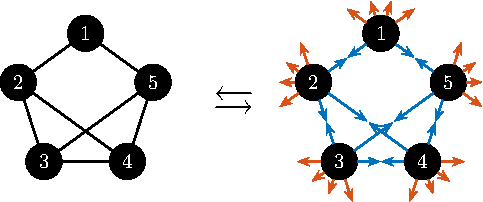
\includegraphics[width=\columnwidth]{../main/fr_layout/fr_layout1.pdf}
          \caption*{\large{$w_{i,j} > 0 \iff \{i,j\} \in E$}}
        \end{figure}
      \end{column}
      \begin{column}{0.5\columnwidth}
        \begin{figure}[h]
          \centering
          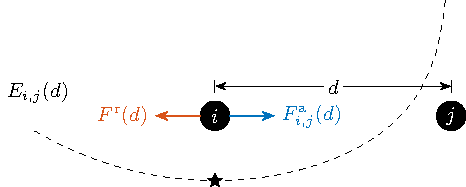
\includegraphics[width=\columnwidth]{../main/fr_layout/fr_layout2.pdf}
          \caption*{\large{$d = \norm{x_i - x_j}$}}
        \end{figure}
      \end{column}
    \end{columns}
  \end{frame}
\fi

\ifShowHidden
  \begin{frame}{``Twist'' Causes Stagnation}
    \large{%
      \textbf{Twist}: unnecessary folded and tangled structures~\cite{veldhuizenDynamicMultilevelGraph2007,cheongSnapshotVisualizationComplex2018}.\\
      $\to$ Causing stagnation of the simulation process.\\
      Slow for large-scale graphs. $\order{\abs{V}^2}$ per iteration.
    }
    \begin{figure}[htbp]
      \centering
      \animategraphics[autoplay,loop,width=0.4\columnwidth]{5}{circle/circle-}{1}{50}%!!!50
    \end{figure}
  \end{frame}
\fi

\ifShowHidden
  \begin{frame}{Previous Works (1/2) - L-BFGS}
    \begin{columns}
      \begin{column}{0.6\columnwidth}
        \large{\textbf{L-BFGS (Quasi-Newton Method)}}~\cite{6183577}\\
        \quad Numerical optimization approach.\\
        \quad Overcome ``twist'' issues to some extent.\\
        \quad Effective for reducing stress.\\[1.5em]
        \textbf{Limitations}\\
        \quad May fail to achieve the optimal visualization.\\
        \quad Flatten the matrix $X$ to a vector $\overline{X}$.\\
        \quad Start from \textbf{a random initial placement}.\\[1.5em]
        \textbf{\red{Our Aim}}\\
        \quad \red{Accelerate by improving initial placement.}\\
      \end{column}
      \begin{column}{0.4\columnwidth}
        \begin{figure}[htbp]
          \centering
          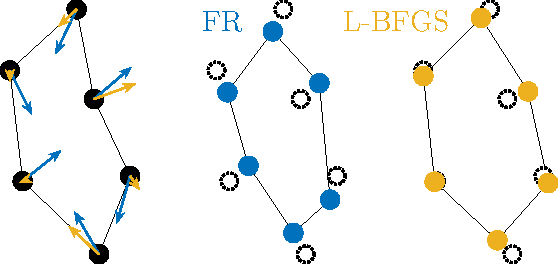
\includegraphics[width=\columnwidth]{../main/comparison/comparison_FRandLBFGS.pdf}
        \end{figure}
        \begin{gather*}
          n\defeq \abs{V}, \quad
          X = \qty( x_1, x_2, \dots, x_n ),\\
          \min_{X \in \bbR^{2\times n}} f(X) \to \min_{\overline{X} \in \bbR^{2n}} \overline{f}(\overline{X})
        \end{gather*}
      \end{column}
    \end{columns}
  \end{frame}
\fi


\ifShowHidden
  \begin{frame}{Previous Works (2/2) - Simulated Annealing}
    \begin{columns}
      \begin{column}{0.5\columnwidth}
        \large{\textbf{Simulated Annealing (SA)}}~\cite{ghassemitoosiSimulatedAnnealingPreProcessing2016}\\
        \quad Providing an initial placement\\
        \quad Effective for addressing ``twist'' issues.\\[1.5em]
        \textbf{Limitations}\\
        \quad Restricted to unweighted graphs.\\
        \quad Limited to circle placement.\\
        \quad Inefficient due to random swapping.\\
        \quad Ignored sparsity of graphs.\\[1.5em]
        \textbf{\red{Our Aim}}\\
        \quad \red{Improve the strategy.}\\
        \quad \red{Extend the applicability.}
      \end{column}
      \begin{column}{0.5\columnwidth}
        \begin{mini*}
          {X \in \bbR^{2 \times n}}
          {\sum_{\{i,j\}\in E \cup E_2} \abs{\angle(x_i, x_j)},}
          {}
          {}
          \addConstraint{x_i}{\in Q^\mathrm{circle} \quad}{\text{for $1 \leq i \leq n$}}
          \addConstraint{x_i}{\neq x_j \quad}{\text{for $1 \leq i < j \leq n$}.}
        \end{mini*}
        \gray{\scriptsize{$Q^\mathrm{circle} \defeq \qty{(\cos(2\pi i/n), \sin(2\pi i/n)) \mid 1 \leq i \leq n}$\\
            $E_2$: a set of vertex pairs with a shortest path distance equal to 2. \textbf{$\abs{E_2}$ could be $\Theta(n^2)$}.\\
            $\angle(a, b)$: the angle between the lines from the origin to the points $a$ and $b$.}}
      \end{column}
    \end{columns}
  \end{frame}
\fi

\ifShowHidden
  \begin{frame}{Our Contribution}
    \begin{figure}[h]
      \centering
      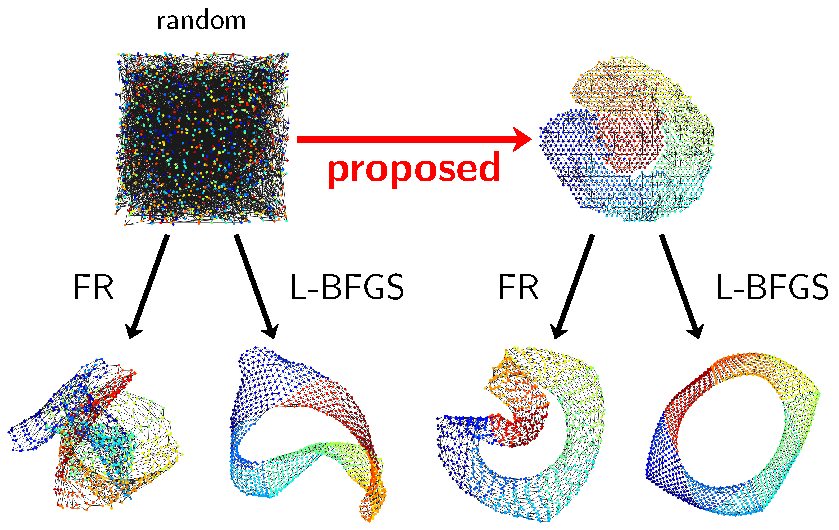
\includegraphics[width=0.75\columnwidth]{../main/fig1/fig1_slide.pdf}
      \caption{\texttt{jagmesh1} dataset after 50 iterations.}
    \end{figure}
  \end{frame}
\fi

\ifShowHidden
  \section{Proposed Method}
\fi

\ifShowHidden
  \begin{frame}{Formulation of the Problem}
    \begin{columns}
      \begin{column}{0.7\columnwidth}
        The two forces in the FR force model:
        \begin{equation*}
          \tccA{F_{i,j}^\mathrm{a}(d) \defeq \frac{w_{i,j} d^2}{k}}, \quad \tccD{F^\mathrm{r}(d) \defeq -\frac{k^2}{d}}.
        \end{equation*}
      \end{column}
      \begin{column}{0.3\columnwidth}
        \vspace{-2.5em}
        \begin{figure}[h]
          \centering
          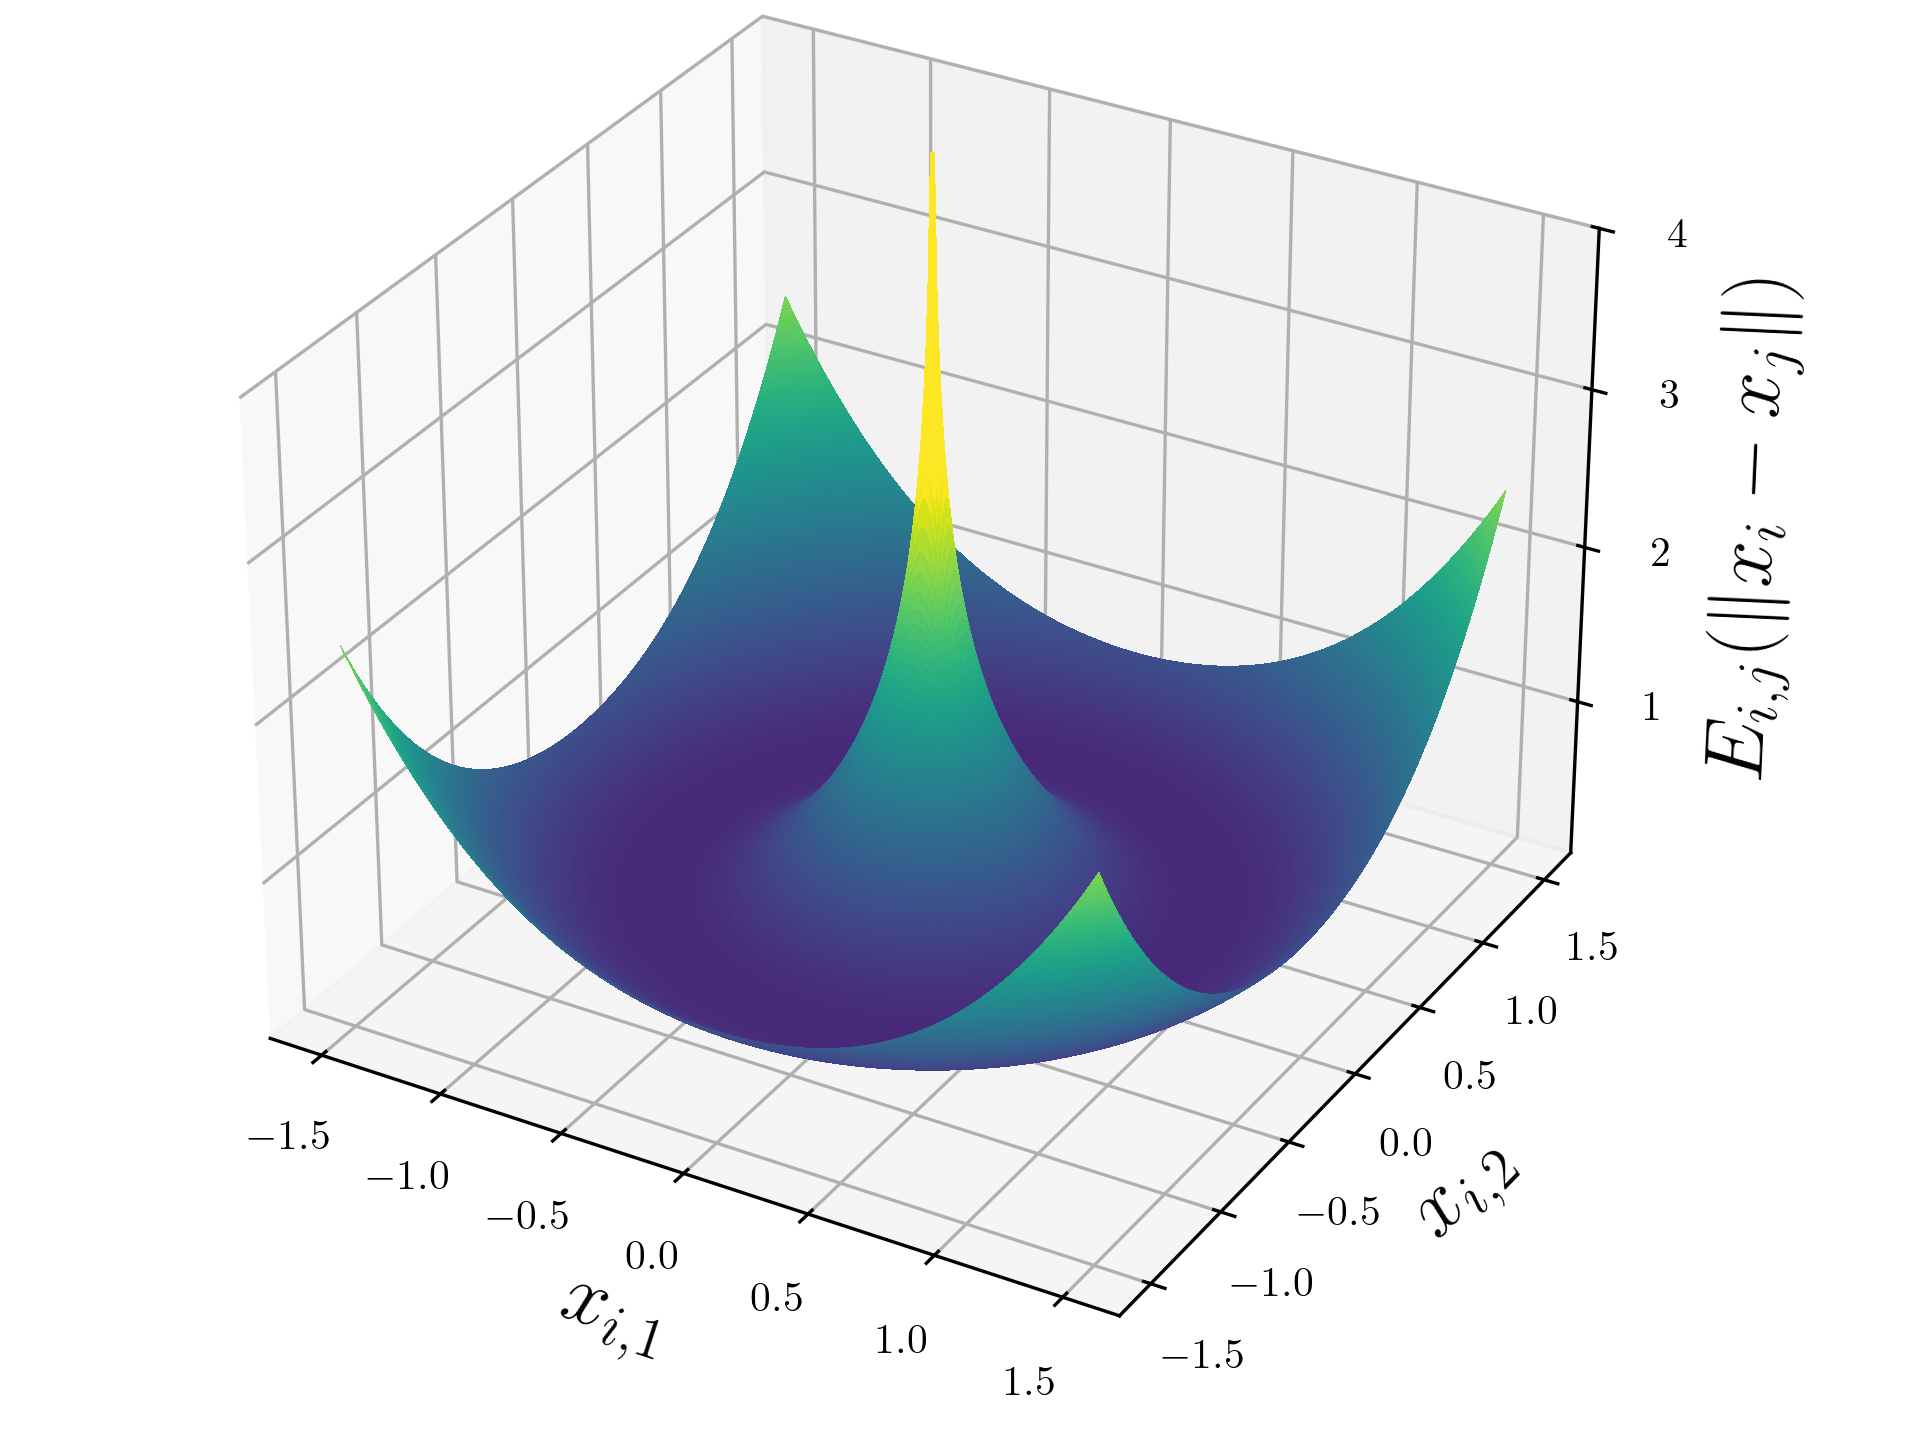
\includegraphics[width=\columnwidth]{../main/energy_3d/energy_3d.png}
        \end{figure}
      \end{column}
    \end{columns}
    Its scalar potential, energy, is defined as
    \begin{gather*}
      \tccA{E_{i,j}^\mathrm{a}(d) \defeq \int_{0}^{d} F_{i,j}^\mathrm{a}(r) \dd{r} = \frac{w_{i,j} d^3}{3k}}, \quad
      \tccD{E^\mathrm{r}(d)       \defeq \int_{\infty}^{d} F^\mathrm{r}(r) \dd{r} = -k^2\log{d}}, \\
      E_{i,j}(d)            \defeq \tccA{E_{i,j}^\mathrm{a}(d)} + \tccD{E^\mathrm{r}(d)}.
    \end{gather*}
    Seek equilibrium $\Leftrightarrow$ \textbf{find local minimum of $f(X)$} (\textbf{non}-convex):
    \begin{mini}
      {X \in \bbR^{2 \times n}}
      {f(X) \defeq \sum_{i<j} E_{i,j}(\norm{x_i - x_j}).}
      {\label{eq:fr}}
      {}
    \end{mini}
  \end{frame}
\fi

\ifShowHidden
  \begin{frame}{Simplify the Problem (1/2)}
    \textbf{Obtain approximated solution quickly.} \quad
    Instead of the problem~\eqref{eq:fr}, we solve:
    \begin{columns}
      \begin{column}{0.55\columnwidth}
        \begin{mini}
          {X \in \bbR^{2 \times n}}
          {\sum_{\{i,j\}\in E} \frac{w_{i,j}\norm{x_i - x_j}^3}{3k},}
          {\label{eq:frApprox0}}
          {}
          \addConstraint{x_i}{\in Q^\mathrm{hex} \quad}{\text{for $1 \leq i \leq n$}}
          \addConstraint{x_i}{\neq x_j \quad}{\text{for $1 \leq i < j \leq n$}.}
        \end{mini}
        where
        \begin{equation*}
          Q^\mathrm{hex} \defeq \left\{ \qty(q+\tfrac{1}{2}r, \tfrac{\sqrt{3}}{2}r) \relmiddle| q \in \bbZ, r \in \bbZ \right\}.
        \end{equation*}
      \end{column}
      \begin{column}{0.45\columnwidth}
        \begin{figure}[t]
          \centering
          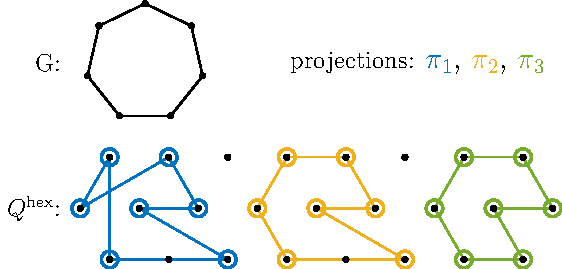
\includegraphics[width=\columnwidth]{../main/pi/pi.pdf}
        \end{figure}
      \end{column}
    \end{columns}

    \vspace{0.3cm}
    \hrulefill\\

    We explain the reason. We simplify the problem~\eqref{eq:fr}. \quad
    Separate $f(X)$ into $\tccA{E^\mathrm{a}_{i,j}}$ and $\tccD{E^\mathrm{r}}$.
    \begin{mini*}
      {X \in \bbR^{2 \times n}}
      {\tccA{\sum_{\{i,j\}\in E} \frac{w_{i,j}\norm{x_i - x_j}^3}{3k}} - \tccD{\sum_{i<j} k^2\log{\norm{x_i - x_j}}}.}
      {}
      {}
    \end{mini*}
  \end{frame}
\fi

\ifShowHidden
  \begin{frame}{Simplify the Problem (2/2)}
    Following previous research, fix the possible positions $x_i$ to a discrete points set $Q$:
    \begin{mini*}
      {X \in \bbR^{2 \times n}}
      {\tccA{\sum_{\{i,j\}\in E} \frac{w_{i,j}\norm{x_i - x_j}^3}{3k}} - \tccD{\sum_{i<j} k^2\log{\norm{x_i - x_j}}},}
      {}
      {}
      \addConstraint{x_i}{\in Q \quad}{\text{for $1 \leq i \leq n$}}
      \addConstraint{x_i}{\neq x_j \quad}{\text{for $1 \leq i < j \leq n$}.}
    \end{mini*}
    $\tccA{\abs{\{\{i,j\} \st \{i,j\} \in E\}} = \abs{E}} \ll \tccD{\abs{\{\{i,j\} \st i<j\}} = \order{\abs{V}^2}}$. Drop the second term.\\
    Take $Q$ such that $\norm{q_i - q_j} \geq \epsilon$ for all $q_i,q_j \in Q (q_i \neq q_j)$.
    Then, the second term is negligible.
    \begin{mini*}
      {X \in \bbR^{2 \times n}}
      {\tccA{f^\mathrm{a}(X) \defeq \sum_{\{i,j\}\in E} \frac{w_{i,j}\norm{x_i - x_j}^3}{3k}},}
      {\label{eq:frApprox2}}
      {}
      \addConstraint{\tccD{x_i}}{\tccD{\in Q \quad}}{\text{for $1 \leq i \leq n$}}
      \addConstraint{\tccD{x_i}}{\tccD{\neq x_j \quad}}{\text{for $1 \leq i < j \leq n$}.}
    \end{mini*}
    Only treat \tccA{\Large{\textbf{a}}}\tccA{ttractive force}. Thus, the points set \tccD{$Q$} should be as dense as possible.\\
    $\to$ \textbf{closet packing} (hexagonal lattice $Q^\mathrm{hex}$).
  \end{frame}
\fi

% \ifShowHidden
\begin{frame}{Summary of the First Half}
  The problem is
  \begin{mini*}
    {X \in \bbR^{2 \times n}}
    {f(X) \defeq \sum_{i<j} E_{i,j}(\norm{x_i - x_j}) = \tccA{\sum_{\{i,j\}\in E} \frac{w_{i,j}\norm{x_i - x_j}^3}{3k}} - \tccD{\sum_{i<j} k^2\log{\norm{x_i - x_j}}}. \tag{\ref{eq:fr}}}
    {}
    {}
  \end{mini*}
  \begin{columns}
    \begin{column}{0.55\columnwidth}
      We simplify the problem as
      \begin{mini*}
        {X \in \bbR^{2 \times n}}
        {\tccA{f^\mathrm{a}(X) \defeq \sum_{\{i,j\}\in E} \frac{w_{i,j}\norm{x_i - x_j}^3}{3k}}, \tag{\ref{eq:frApprox0}}}
        {}
        {}
        \addConstraint{\tccD{x_i}}{\tccD{\in Q^\mathrm{hex} \quad}}{\text{for $1 \leq i \leq n$}}
        \addConstraint{\tccD{x_i}}{\tccD{\neq x_j \quad}}{\text{for $1 \leq i < j \leq n$}.}
      \end{mini*}
    \end{column}
    \begin{column}{0.45\columnwidth}
      \begin{figure}[t]
        \centering
        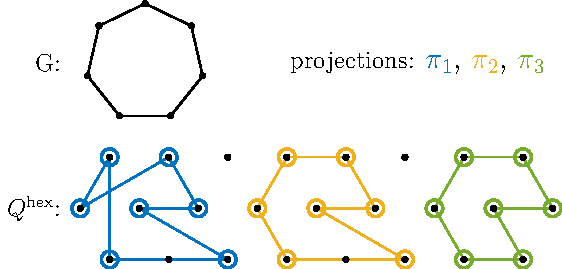
\includegraphics[width=\columnwidth]{../main/pi/pi.pdf}
      \end{figure}
    \end{column}
  \end{columns}
  We will explain how to solve in the second half.
\end{frame}
% \fi

% \ifShowHidden
\begin{frame}{Base of Proposed Algorithm - Stochastic Coordinate Descent}
  Let $f\colon \bbR^n \to \bbR$ be strictly convex. The second order approximation at $x_0$ is
  \begin{equation*}
    f(x) \approx f(x_0) + \nabla f(x_0)^\top (x - x_0) + \frac{1}{2} (x - x_0)^\top \nabla^2 f(x_0) (x - x_0).
  \end{equation*}
  The minimum $x^*$ satisfies
  \begin{align*}
         & \nabla f(x_0) + \nabla^2 f(x_0) (x^* - x_0) = 0                                                       \\
    \iff & x^* = x_0 \red{- \nabla^2 f(x_0)^{-1} \nabla f(x_0)}. \qquad \text{\textbf{\red{(Newton direction)}}}
  \end{align*}
  Although it is effective, computing the Newton direction is \textbf{too expensive}...\\[1em]

  We use the \large{\textbf{stochastic coordinate descent}} with the \large{\textbf{\red{coordinate Newton direction}}}.\\
  Let $f_i(x_i)$ be the limitation to the $i$-th coordinate (randomly selected).\\
  The coordinate Newton direction: $d_i = -\nabla^2 f_i(x_i)^{-1} \nabla f_i(x_i)$. \red{$\leftarrow$ \large{\textbf{Cheap! Computable!}}}
\end{frame}
% \fi

% \ifShowHidden
\begin{frame}{Proposed Algorithm (1/3) - Coordinate Newton Direction}
  We solve the problem~\eqref{eq:frApprox0} using \textbf{the coordinate Newton direction.}

  Let $f^{\mathrm{a}}_i(x_i)$ corresponding to a vertex $v_i$ be
  \begin{equation*}
    f^{\mathrm{a}}_i(x_i) \defeq \sum_{j \neq i} \frac{w_{i,j}\norm{x_i - x_j}^3}{3k}.
  \end{equation*}
  Its gradient and Hessian matrix are
  \begin{align*}
    \nabla f^{\mathrm{a}}_i(x_i)   & = \sum_{j \neq i} \frac{w_{i,j}\norm{x_i - x_j}}{k} (x_i - x_j),     \\
    \nabla^2 f^{\mathrm{a}}_i(x_i) & = \sum_{j \neq i} \frac{w_{i,j}\norm{x_i - x_j}}{k} \mqty(1      & 0 \\0&1) + \sum_{j \neq i} \frac{w_{i,j}}{k\norm{x_i - x_j}} (x_i - x_j)(x_i - x_j)^\top.
  \end{align*}
  $f^{\mathrm{a}}_i$ is \textbf{strictly convex}.
  Different from $E_{i,j}(\norm{\cdot - x_j})$ in~\eqref{eq:fr} and $f^{\mathrm{a}}(\cdot)$ in~\eqref{eq:frApprox0} (non-convex).
\end{frame}
% \fi

% \ifShowHidden
\begin{frame}{Proposed Algorithm (2/3) - Update Rule}
  Ordinary updated rule:
  \begin{equation*}
    x_i^\mathrm{new} \gets x_i - \nabla^2 f^{\mathrm{a}}_i(x_i)^{-1} \nabla f^{\mathrm{a}}_i(x_i).
  \end{equation*}
  $x_i^\mathrm{new}$ may not be in the hexagonal lattice $Q^\mathrm{hex}$.
  Need rounding to the nearest point in $Q^\mathrm{hex}$.\\
  We empirically found that adding a random noise is effective.
  \begin{equation*}
    x_i^\mathrm{new} \gets \mathrm{round}\qty(x_i - \nabla^2 f^{\mathrm{a}}_i(x_i)^{-1} \nabla f^{\mathrm{a}}_i(x_i) + t \cdot \text{rand}),
  \end{equation*}
  ($\mathrm{round}(\hat{x})$: the operation assigning $\hat{x}$ to the nearest point in $Q^\mathrm{hex}$,\\
  $\mathrm{rand}$ is a random vector with a unit norm, and $t$ is a parameter controlling the randomness.)

  \begin{figure}[t]
    \centering
    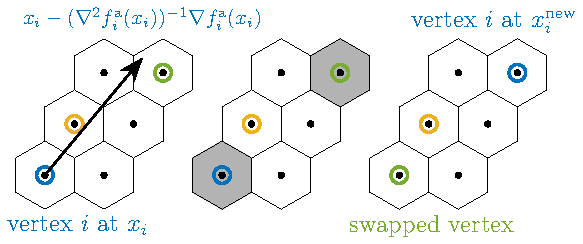
\includegraphics[width=0.5\columnwidth]{../main/hex/hex.pdf}
    \label{fig:hex}
  \end{figure}
\end{frame}
% \fi

% \ifShowHidden
\begin{frame}{Proposed Algorithm (3/3) - Optimal Scaling}
  \begin{columns}
    \begin{column}{0.75\columnwidth}
      We can find optimal scaling factor $\red{c^*}$.
      We scale $X = (x_1, \dots, x_n)$ as $x_i \gets c x_i$ for all $i$.
      This problem is to minimize $\phi(c)$:
      \begin{equation*}
        \phi(c) \defeq \qty(\sum_{\{i,j\} \in E} \frac{w_{i,j} (\red{c} \norm{x_i - x_j})^3}{3k}) - k^2 \sum_{i < j} \log(\red{c} \norm{x_i - x_j})
      \end{equation*}
      $\phi(c)$ is convex, and the optimal scaling factor $\red{c^*}$ by
      \begin{equation}\label{eq:scaling}
        \red{c^*} = \qty(\frac{k^2 n(n-1)}{2 \sum_{\{i,j\} \in E} \frac{w_{i,j} \norm{x_i - x_j}^3}{k}})^{1/3}.
      \end{equation}
      This value can be computed in the \text{$\order{\abs{E}}$ complexity}.

      As far as we rescale the placement by $\red{c^*}$,\\
      \textbf{we don't need to care $\epsilon$} to define $Q (\norm{q_i - q_j} \geq \epsilon)$.
    \end{column}
    \begin{column}{0.25\columnwidth}
      \vspace{-0.5cm}
      \begin{figure}[t]
        \centering
        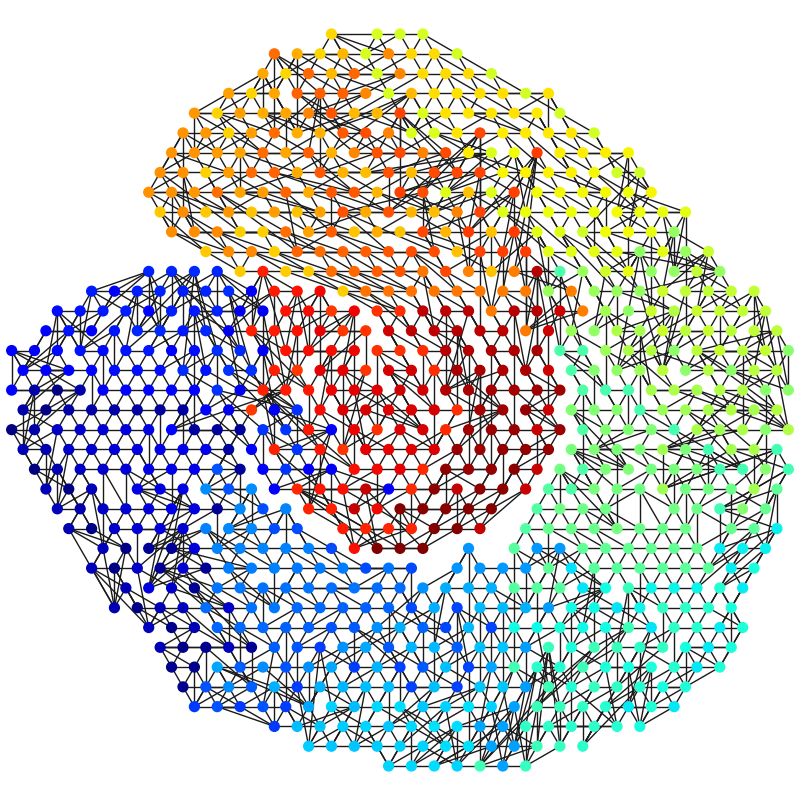
\includegraphics[width=0.2\columnwidth]{../main/individual/vis/fig1_init_CN.png}\\
        \begin{tikzpicture}
          \draw[->, thick] (0, 0.5) -- (0, 0) node[midway, right] {$\times \red{c^*}$} node[midway, left] {\phantom{$\times c^*$}};
        \end{tikzpicture}
        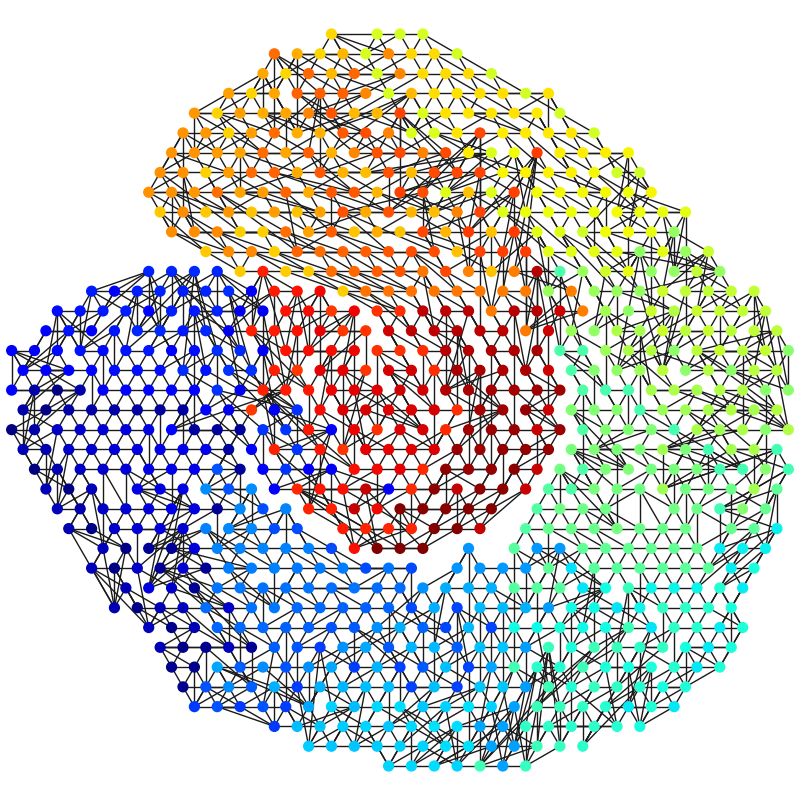
\includegraphics[width=0.8\columnwidth]{../main/individual/vis/fig1_init_CN.png}\\
        
\begin{tikzpicture}
          \draw[->, thick] (0, 0.5) -- (0, 0) node[midway, right] {L-BFGS} node[midway, left] {\phantom{L-BFGS}};
        \end{tikzpicture}
        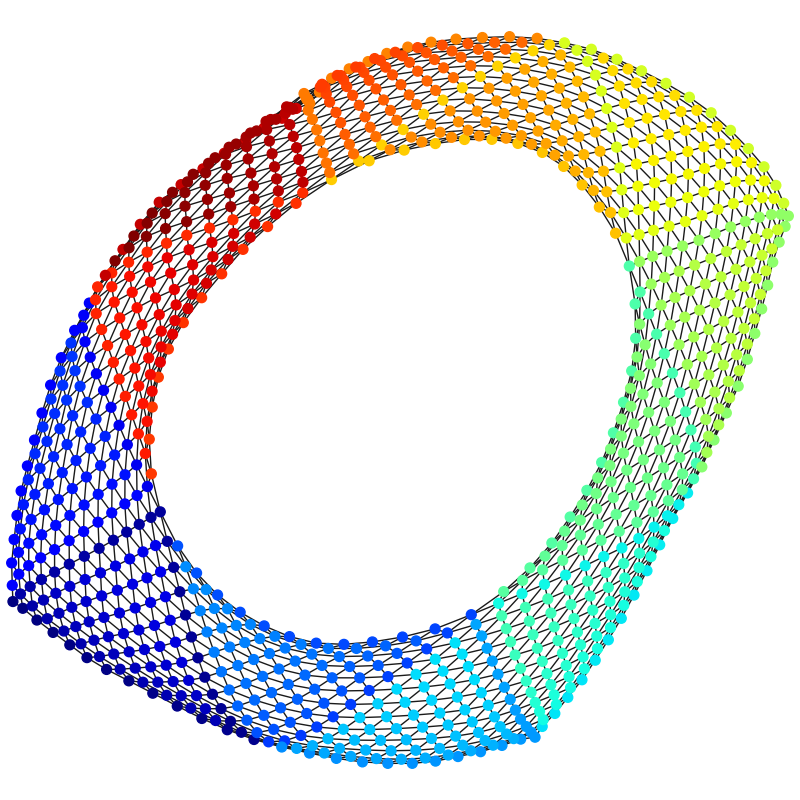
\includegraphics[width=0.8\columnwidth]{../main/individual/vis/jagmesh1_CN-L-BFGS.png}
      \end{figure}
    \end{column}
  \end{columns}
\end{frame}
% \fi

% \ifShowHidden
\begin{frame}[fragile]{Pseudo Code}
  \begin{center}
    \begin{minipage}{0.88\columnwidth}
      \vspace{-0.2cm}
      \begin{algorithm}[H]
        \caption{Proposed algorithm as initial placement}
        \label{alg:proposed}
        \KwIn{Graph $G = (V, E)$, Weight $(w_{i,j})_{\qty{i,j} \in E}$, Parameters $N_\mathrm{iter}^\mathsf{CN}\in\bbN,$ $t_0>0$}
        \KwOut{Initial placement $X = (x_1, \dots, x_n)$}
        $t \gets t_0$\;
        Sample $x_i \in Q$ for all $i \in V$ without replacement\;
        \For{$m \gets 0$ \KwTo $N_\mathrm{iter}^\mathsf{CN}$}{
        Select vertex $i \in V$ randomly\;
        $x_i^\mathrm{new} \gets \mathrm{round}(x_i - \nabla^2 f_i(x_i)^{-1} \nabla f_i(x_i) + t \cdot \mathrm{rand})$\;
          \If{$\exists j \in V \st x_j = x_i^\mathrm{new}$}{
            Swap $x_i$ and $x_j$\;
          } \Else{
            $x_i \gets x_i^\mathrm{new}$\;
          }
          $t \gets t - t_0 / N_\mathrm{iter}^\mathsf{CN}$\;
          }
        $x_i \gets c^* x_i$ for all $i \in V$ with $c^*$ by Eq.\eqref{eq:scaling}\;
          \Return $X$
      \end{algorithm}
    \end{minipage}
  \end{center}
\end{frame}
% \fi

\section{Experiments}

\ifShowHidden
  \begin{frame}{Experiments Result (gif)}
    \begin{figure}[htbp]
      \centering
      \animategraphics[loop,width=0.4\columnwidth]{5}{jagmesh1/CN-L-BFGS/}{0}{67}%!!!111
    \end{figure}
  \end{frame}
\fi

\ifShowHidden
  \begin{frame}{Experiments Result (individual 1)}
    \begin{figure}[h]
      \centering
      \addtolength{\tabcolsep}{-0.5em}
      \begin{tabular}{cccccc}
        \multicolumn{6}{c}{\textbf{\texttt{jagmesh1}} $(\abs{V}=936, \abs{E}=2664, \text{sparsity}=0.609\text{\%})$ \quad Figures are at 50 iterations.}    \\
        \raisebox{-.5\height}{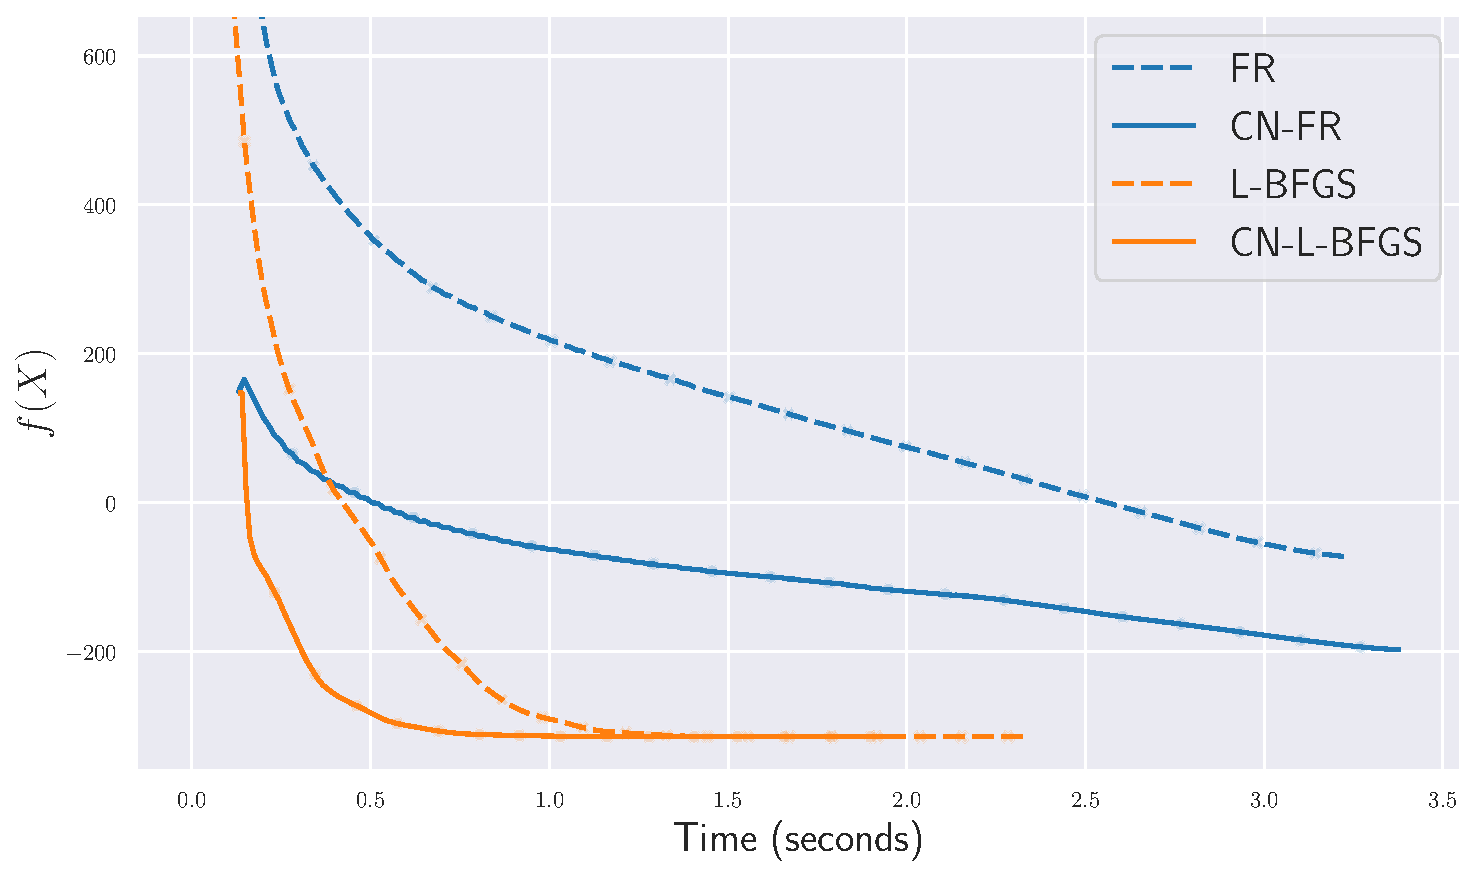
\includegraphics[width=0.275\columnwidth]{../main/individual/plot/jagmesh1.pdf}} &
        \makecell{\small{\textsf{FR}}                                                                                                                       \\[-0.2em]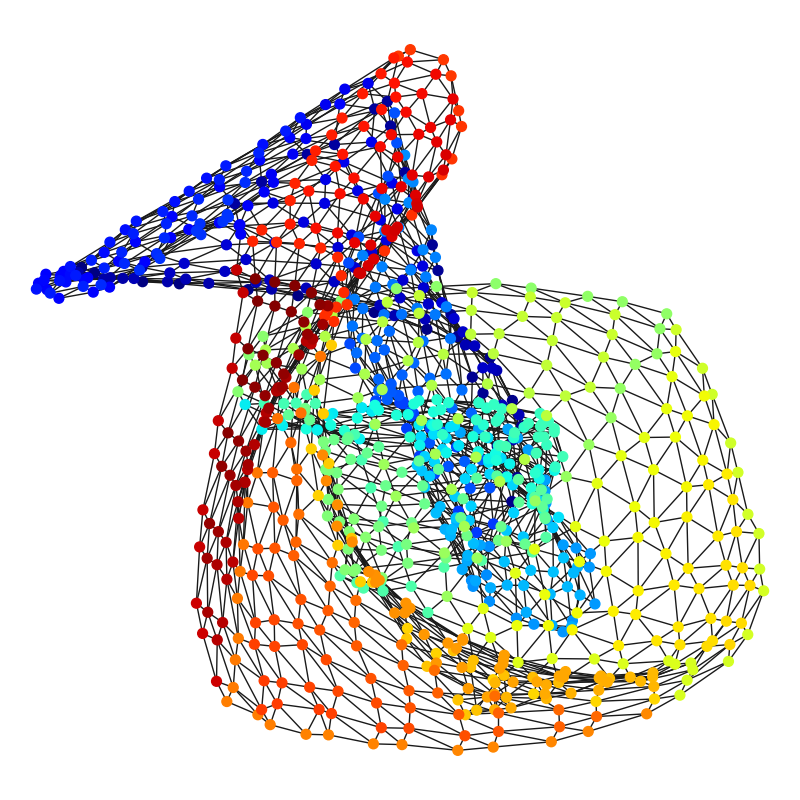
\includegraphics[width=0.135\columnwidth]{../main/individual/vis/jagmesh1_FR.png}} &
        \makecell{\small{\textsf{L-BFGS}}                                                                                                                   \\[-0.2em]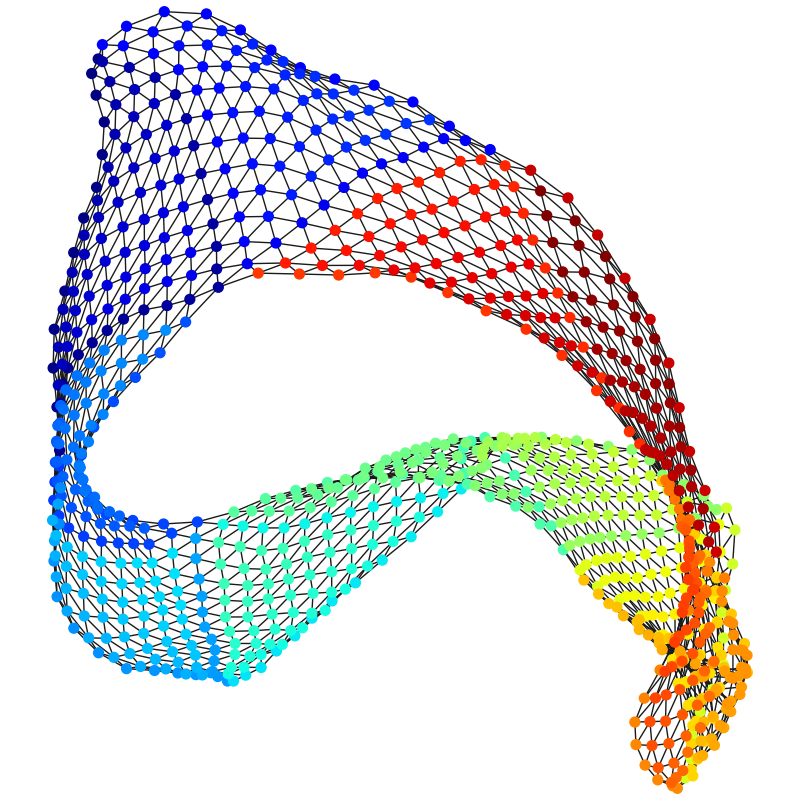
\includegraphics[width=0.135\columnwidth]{../main/individual/vis/jagmesh1_L-BFGS.png}} &
        \makecell{\small{\textsf{\textbf{CN}-FR}}                                                                                                           \\[-0.2em]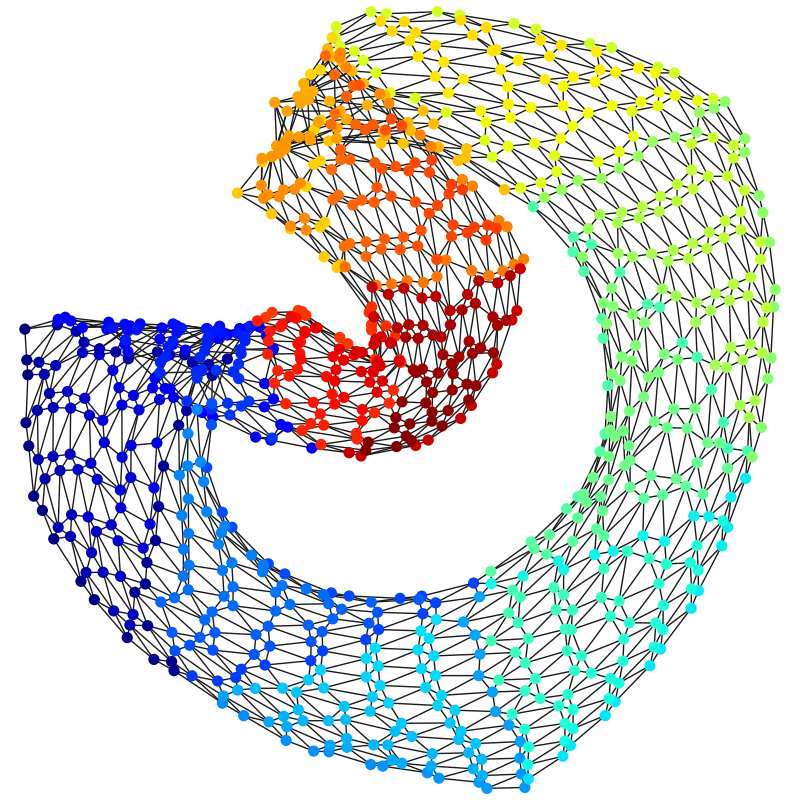
\includegraphics[width=0.135\columnwidth]{../main/individual/vis/jagmesh1_CN-FR.png}} &
        \makecell{\small{\textsf{\textbf{CN}-L-BFGS}}                                                                                                       \\[-0.2em]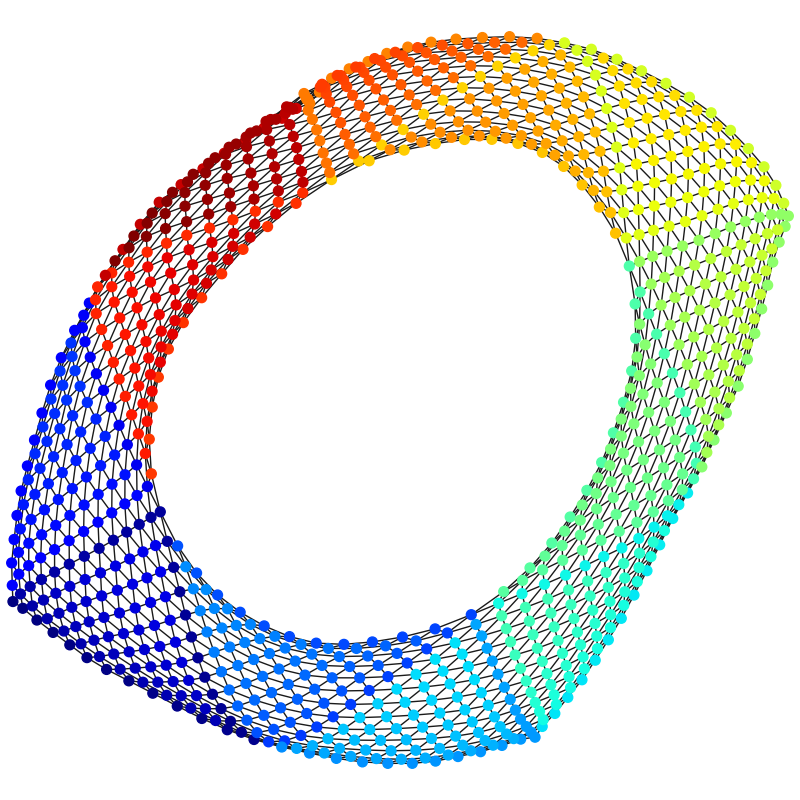
\includegraphics[width=0.135\columnwidth]{../main/individual/vis/jagmesh1_CN-L-BFGS.png}} &
        \makecell{\small{\textsf{BEST}}                                                                                                                     \\[-0.2em]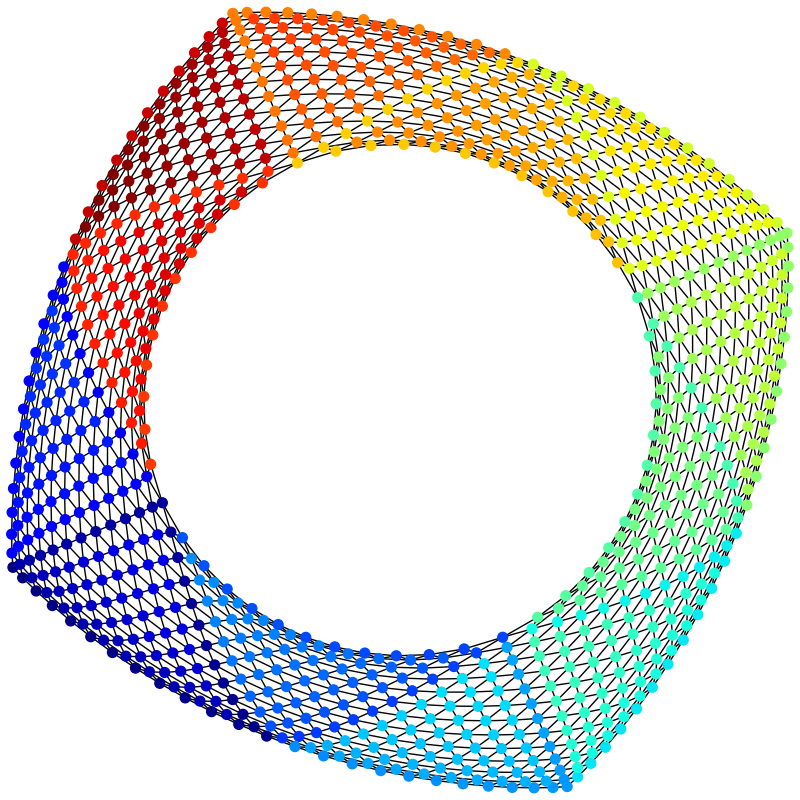
\includegraphics[width=0.135\columnwidth]{../main/individual/vis/opt_jagmesh1.png}} \\

        \multicolumn{6}{c}{\textbf{\texttt{dwt\_1005}} $(\abs{V}=1005, \abs{E}=3808, \text{sparsity}=0.755\text{\%})$ \quad Figures are at 100 iterations.} \\
        \raisebox{-.5\height}{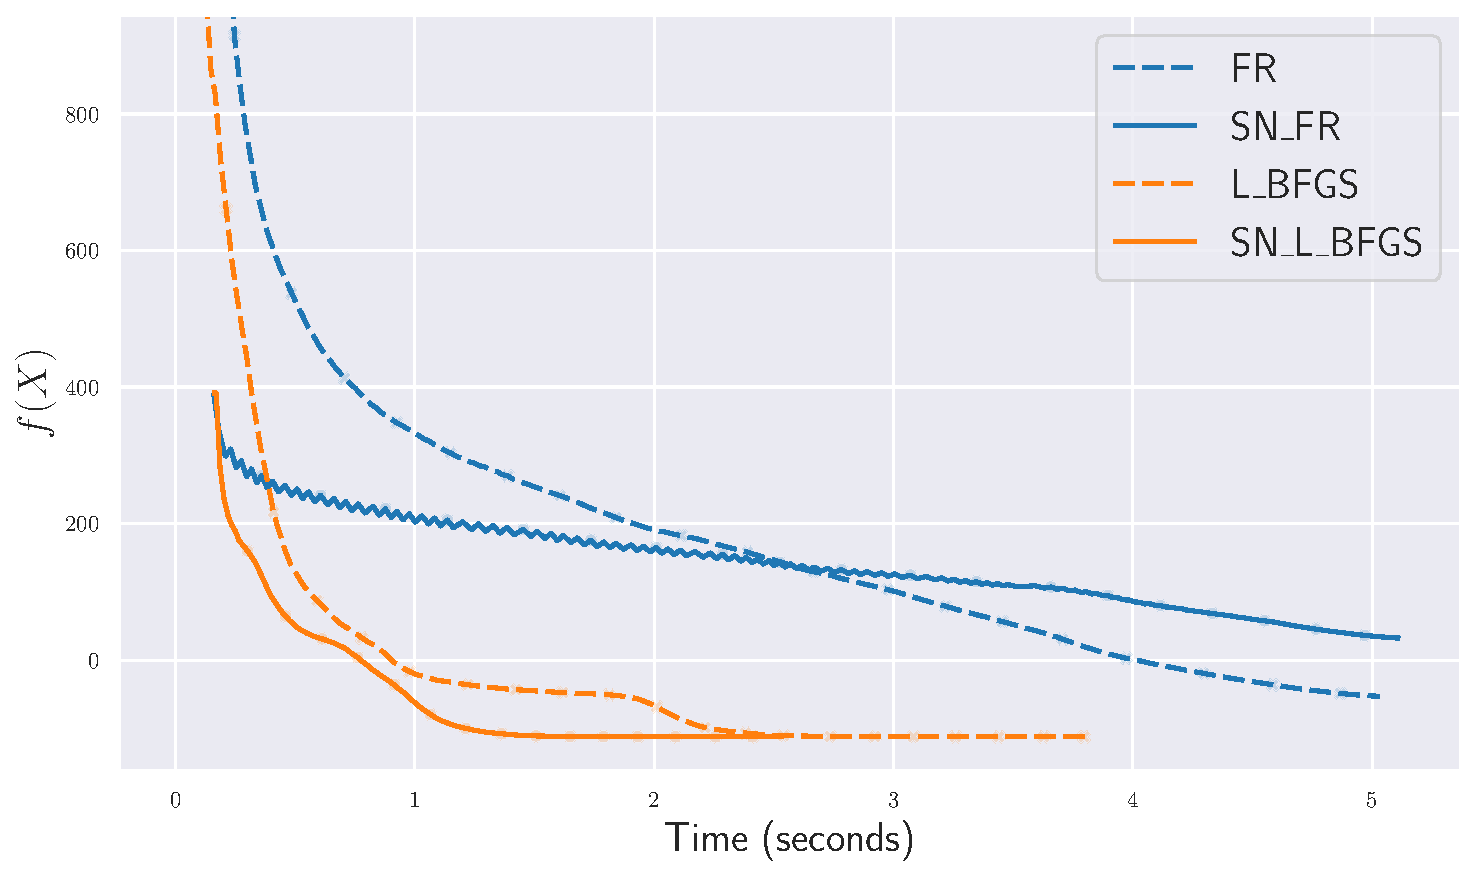
\includegraphics[width=0.275\columnwidth]{../main/individual/plot/dwt_1005.pdf}} &
        \makecell{\small{\textsf{FR}}                                                                                                                       \\[-0.2em]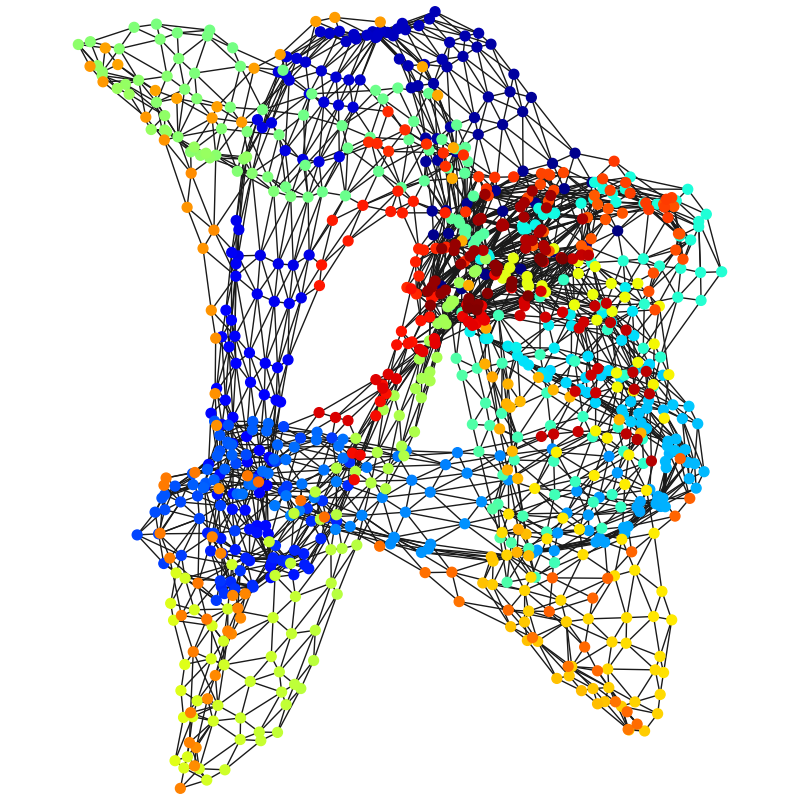
\includegraphics[width=0.135\columnwidth]{../main/individual/vis/dwt_1005_FR.png}} &
        \makecell{\small{\textsf{L-BFGS}}                                                                                                                   \\[-0.2em]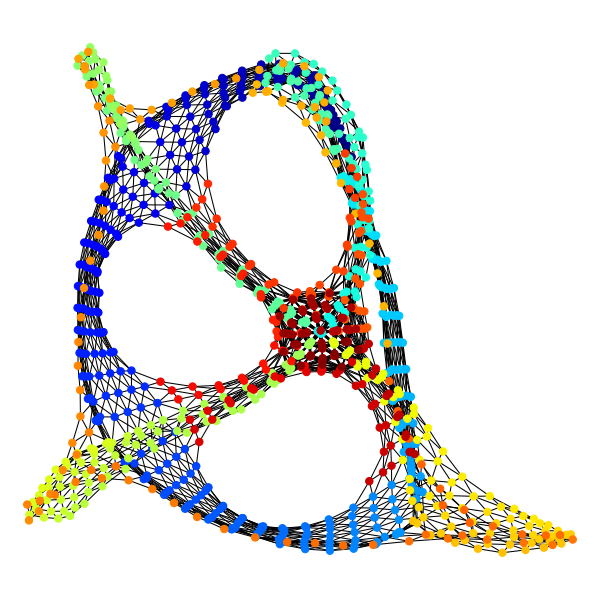
\includegraphics[width=0.135\columnwidth]{../main/individual/vis/dwt_1005_L-BFGS.png}} &
        \makecell{\small{\textsf{\textbf{CN}-FR}}                                                                                                           \\[-0.2em]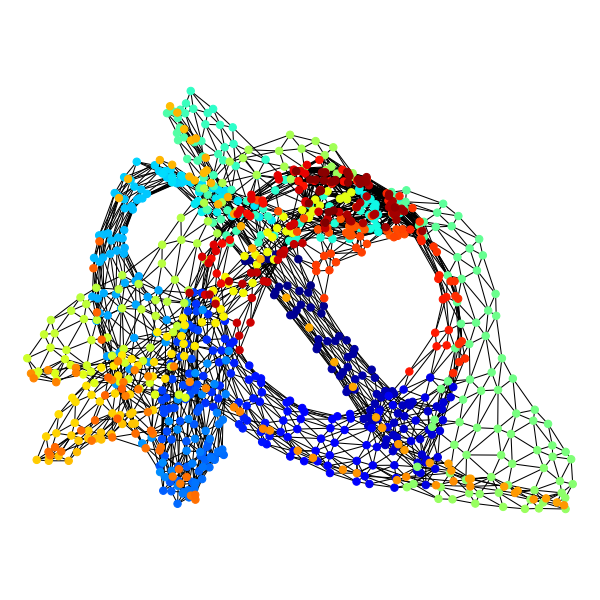
\includegraphics[width=0.135\columnwidth]{../main/individual/vis/dwt_1005_CN-FR.png}} &
        \makecell{\small{\textsf{\textbf{CN}-L-BFGS}}                                                                                                       \\[-0.2em]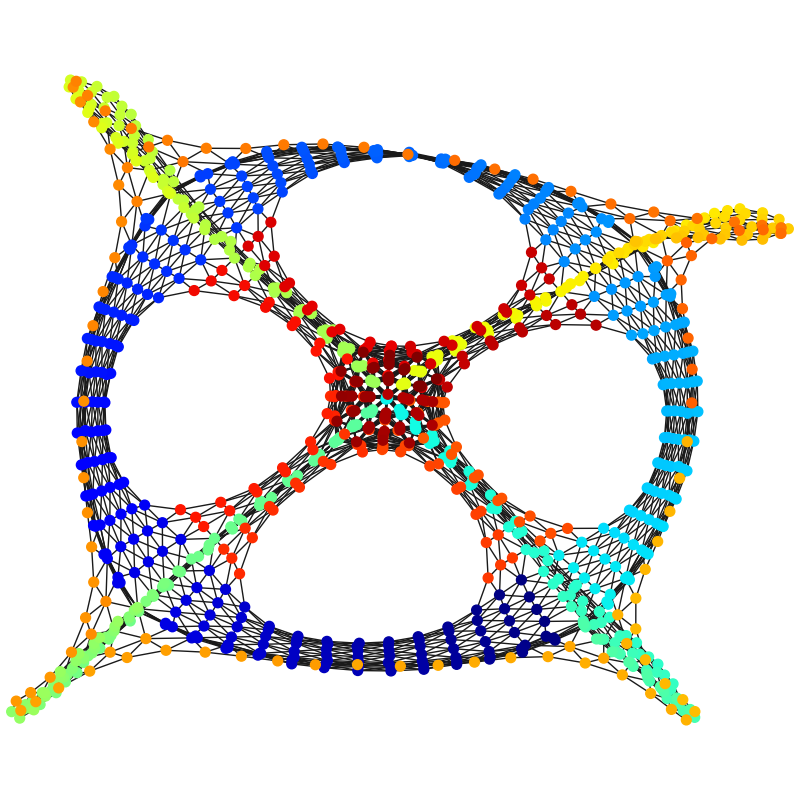
\includegraphics[width=0.135\columnwidth]{../main/individual/vis/dwt_1005_CN-L-BFGS.png}} &
        \makecell{\small{\textsf{BEST}}                                                                                                                     \\[-0.2em]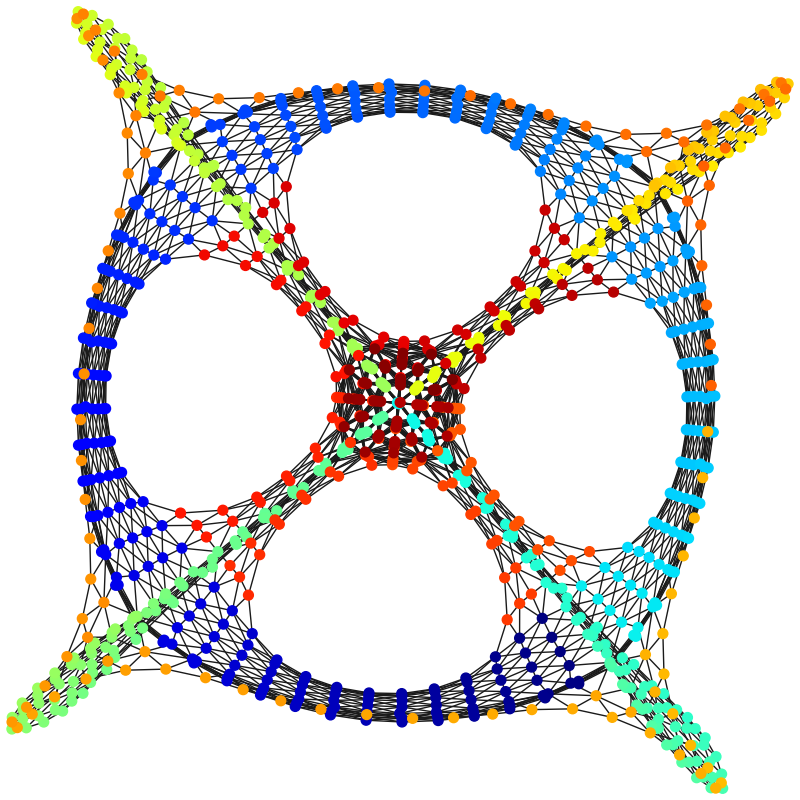
\includegraphics[width=0.135\columnwidth]{../main/individual/vis/opt_dwt_1005.png}} \\
      \end{tabular}
      \caption{``BEST'' is the 500th iteration of the proposed algorithm.}
    \end{figure}
  \end{frame}
\fi

\ifShowHidden
  \begin{frame}{Experiments Result (individual 2)}
    \begin{figure}[h]
      \centering
      \addtolength{\tabcolsep}{-0.5em}
      \begin{tabular}{cccccc}
        \multicolumn{6}{c}{\textbf{\texttt{dwt\_2680}} $(\abs{V}=2680, \abs{E}=11173, \text{sparsity}=0.311\text{\%})$ \quad Figures are at 150 iterations.} \\
        \raisebox{-.5\height}{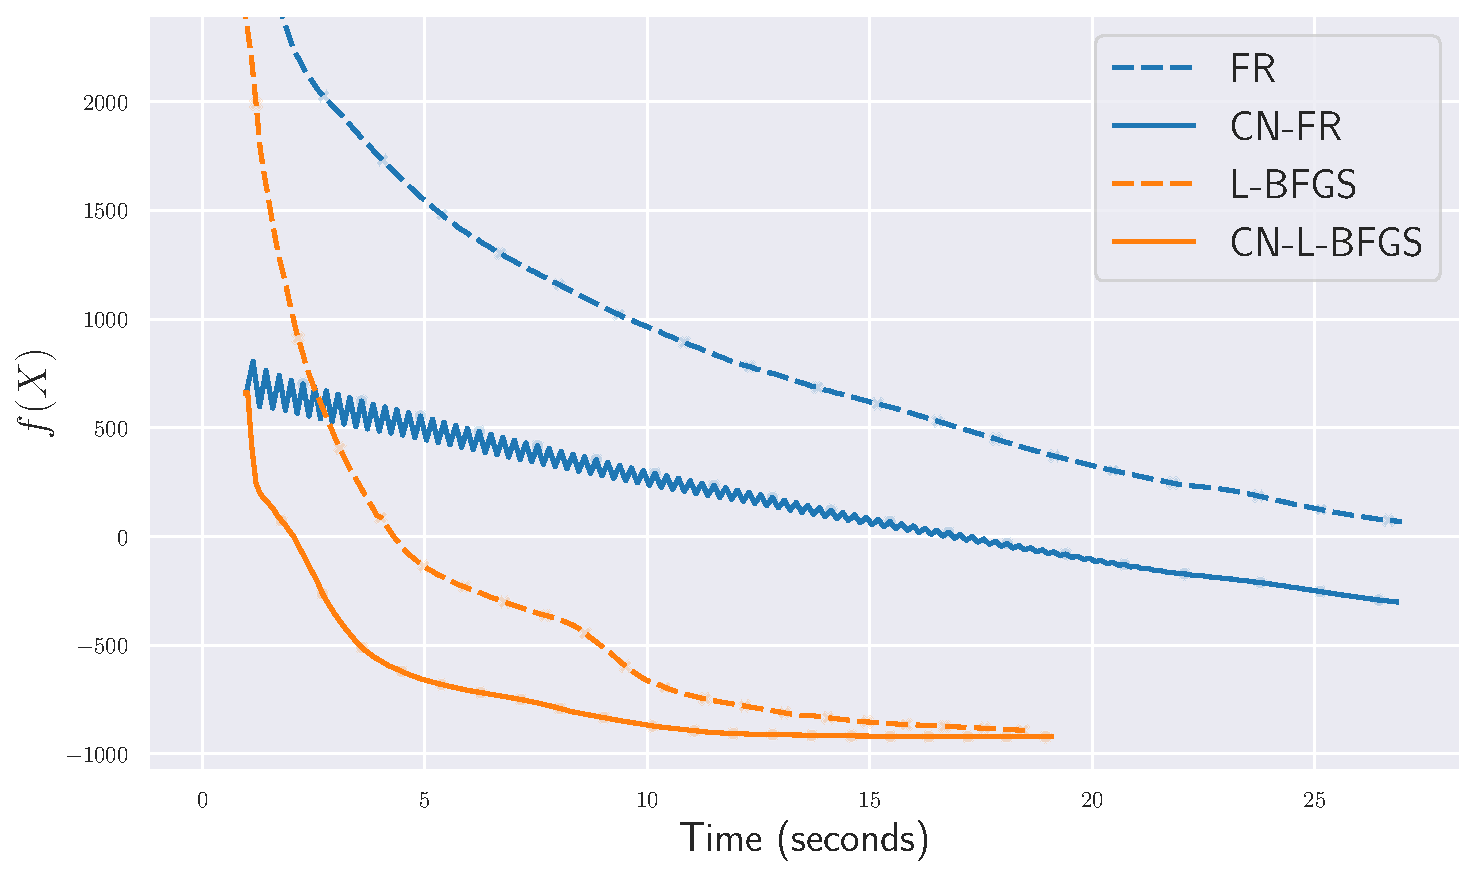
\includegraphics[width=0.275\columnwidth]{../main/individual/plot/dwt_2680.pdf}} &
        \makecell{\small{\textsf{FR}}                                                                                                                        \\[-0.2em]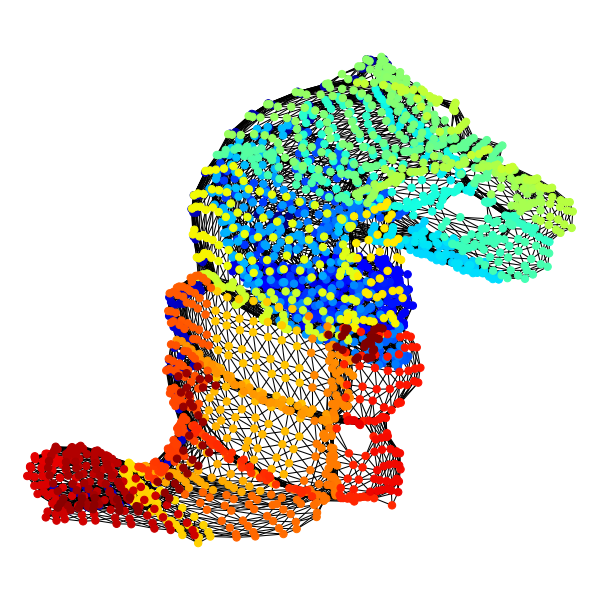
\includegraphics[width=0.135\columnwidth]{../main/individual/vis/dwt_2680_FR.png}} &
        \makecell{\small{\textsf{L-BFGS}}                                                                                                                    \\[-0.2em]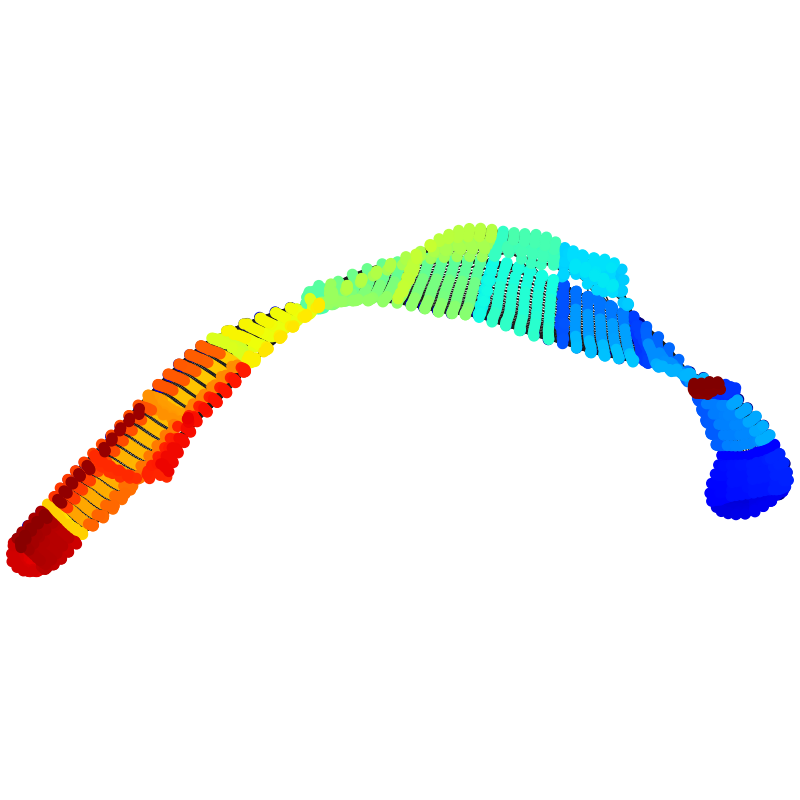
\includegraphics[width=0.135\columnwidth]{../main/individual/vis/dwt_2680_L-BFGS.png}} &
        \makecell{\small{\textsf{\textbf{CN}-FR}}                                                                                                            \\[-0.2em]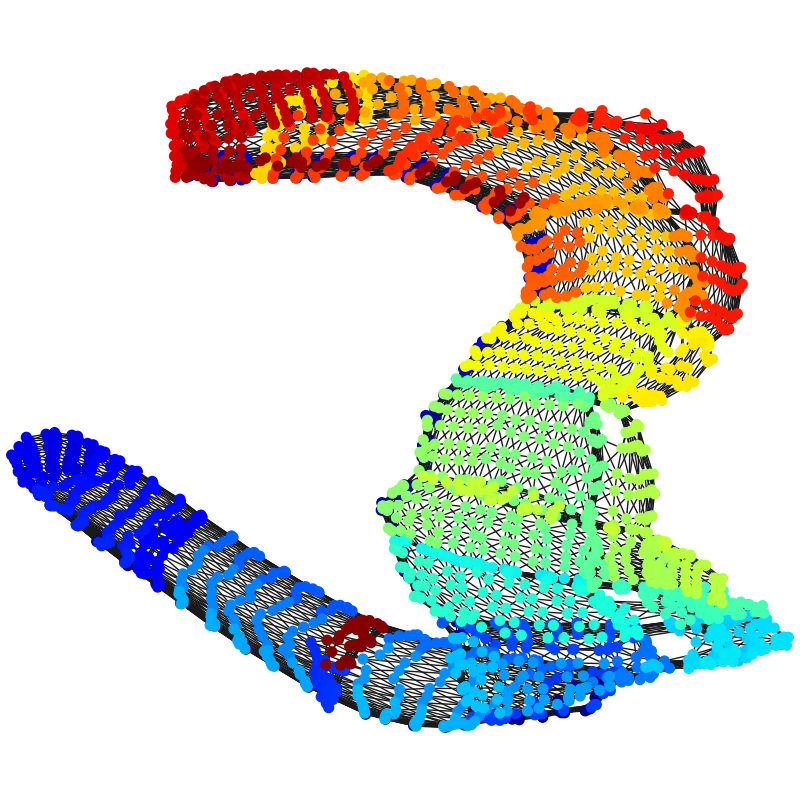
\includegraphics[width=0.135\columnwidth]{../main/individual/vis/dwt_2680_CN-FR.png}} &
        \makecell{\small{\textsf{\textbf{CN}-L-BFGS}}                                                                                                        \\[-0.2em]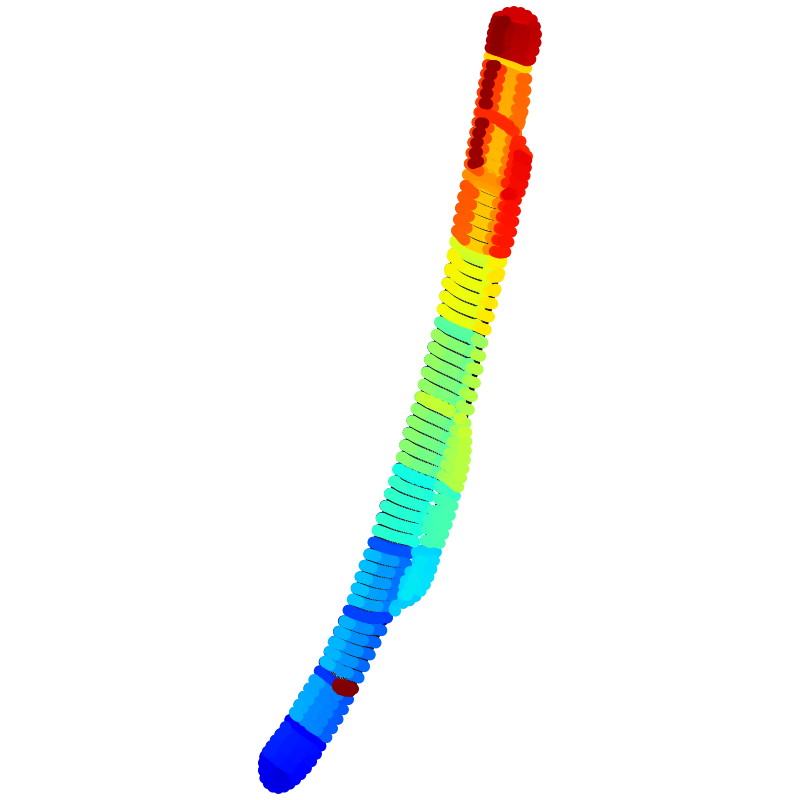
\includegraphics[width=0.135\columnwidth]{../main/individual/vis/dwt_2680_CN-L-BFGS.png}} &
        \makecell{\small{\textsf{BEST}}                                                                                                                      \\[-0.2em]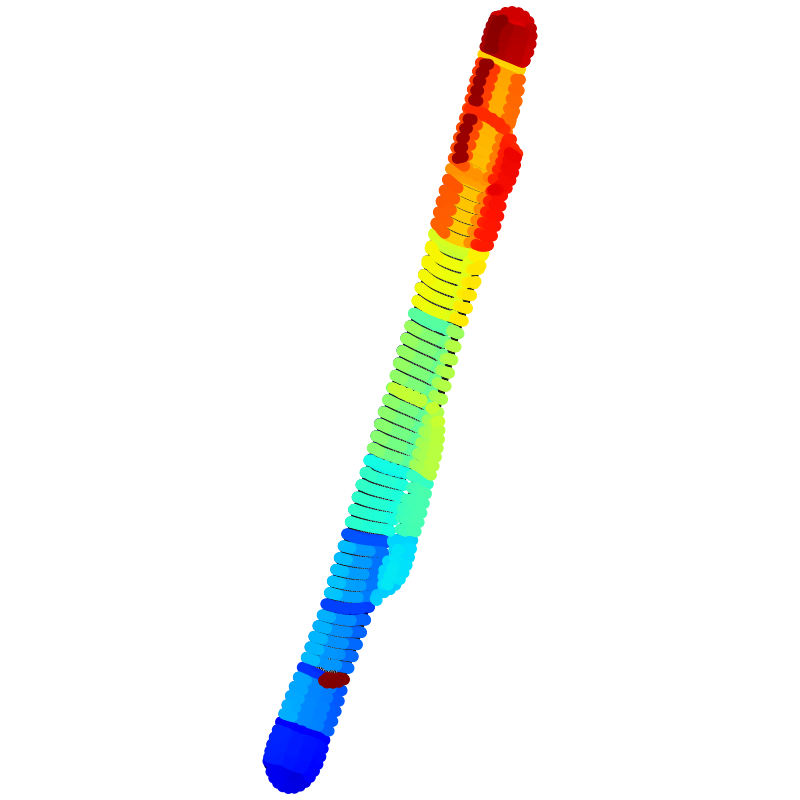
\includegraphics[width=0.135\columnwidth]{../main/individual/vis/opt_dwt_2680.png}} \\

        \multicolumn{6}{c}{\textbf{\texttt{3elt}} $(\abs{V}=4720, \abs{E}=13722, \text{sparsity}=0.123\text{\%})$ \quad Figures are at 150 iterations.}      \\
        \raisebox{-.5\height}{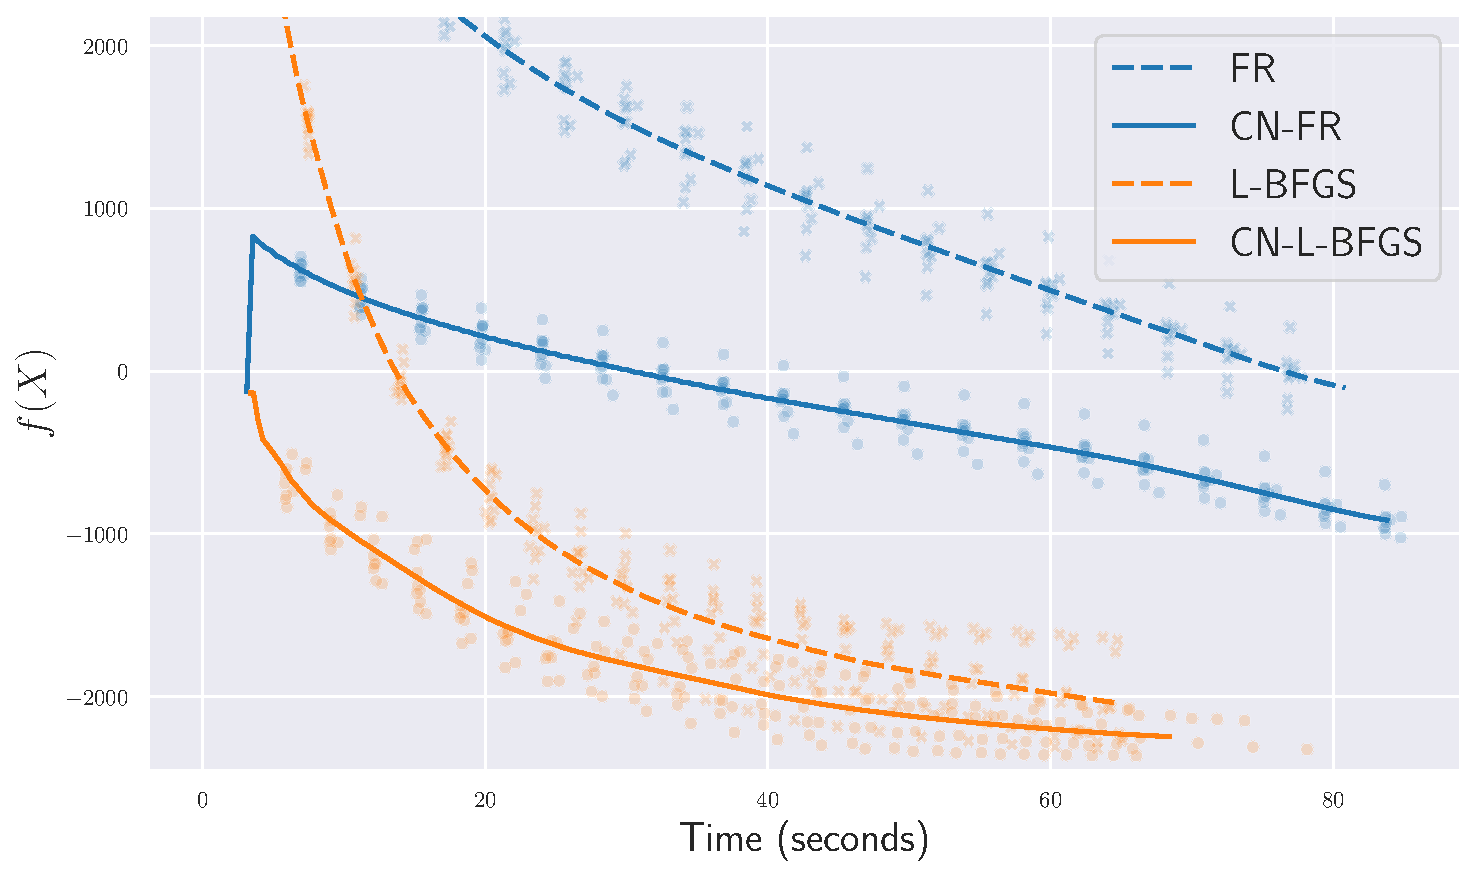
\includegraphics[width=0.275\columnwidth]{../main/individual/plot/3elt.pdf}}     &
        \makecell{\small{\textsf{FR}}                                                                                                                        \\[-0.2em]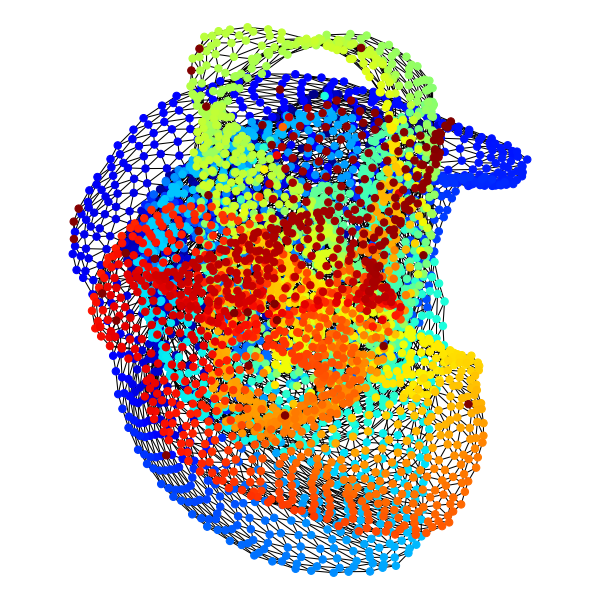
\includegraphics[width=0.135\columnwidth]{../main/individual/vis/3elt_FR.png}} &
        \makecell{\small{\textsf{L-BFGS}}                                                                                                                    \\[-0.2em]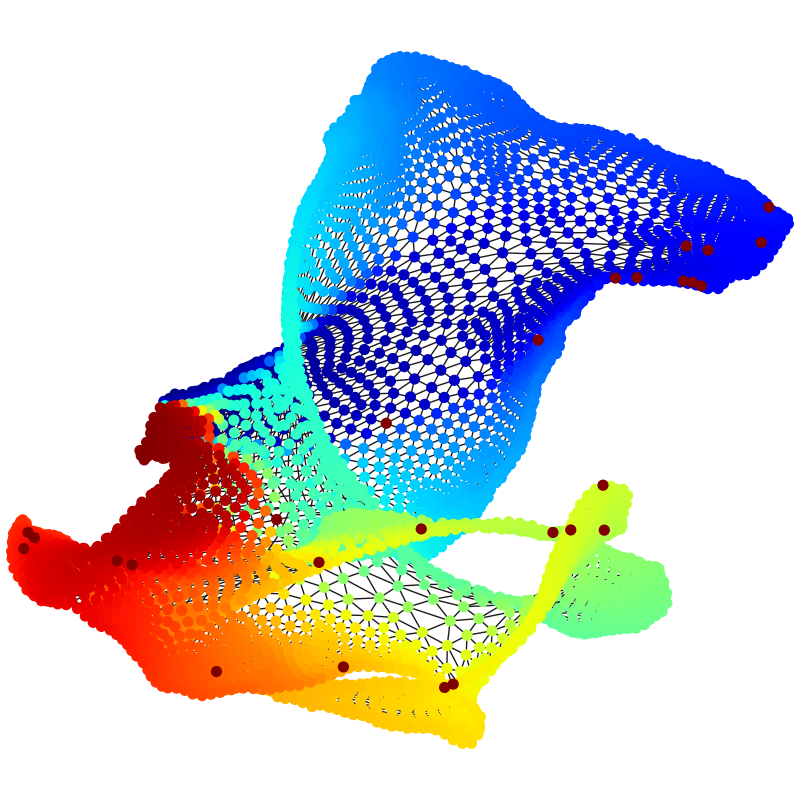
\includegraphics[width=0.135\columnwidth]{../main/individual/vis/3elt_L-BFGS.png}} &
        \makecell{\small{\textsf{\textbf{CN}-FR}}                                                                                                            \\[-0.2em]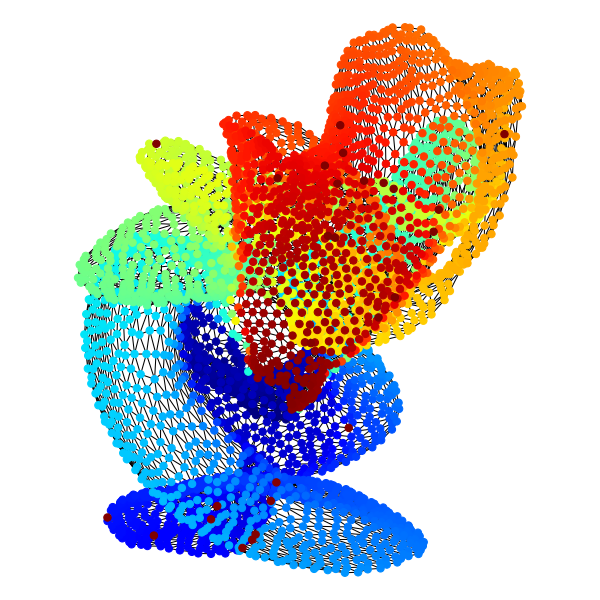
\includegraphics[width=0.135\columnwidth]{../main/individual/vis/3elt_CN-FR.png}} &
        \makecell{\small{\textsf{\textbf{CN}-L-BFGS}}                                                                                                        \\[-0.2em]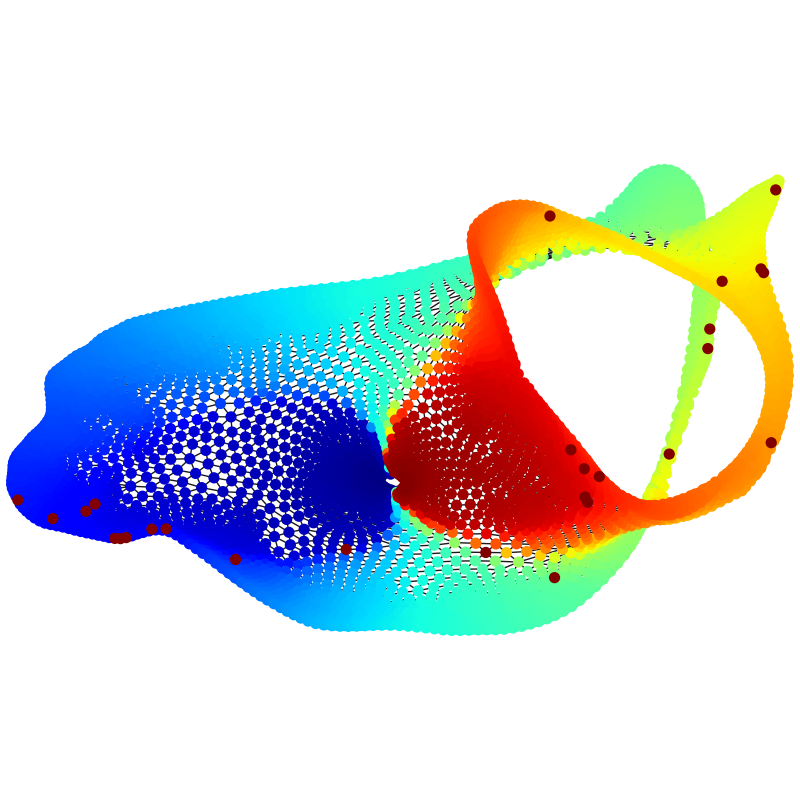
\includegraphics[width=0.135\columnwidth]{../main/individual/vis/3elt_CN-L-BFGS.png}} &
        \makecell{\small{\textsf{BEST}}                                                                                                                      \\[-0.2em]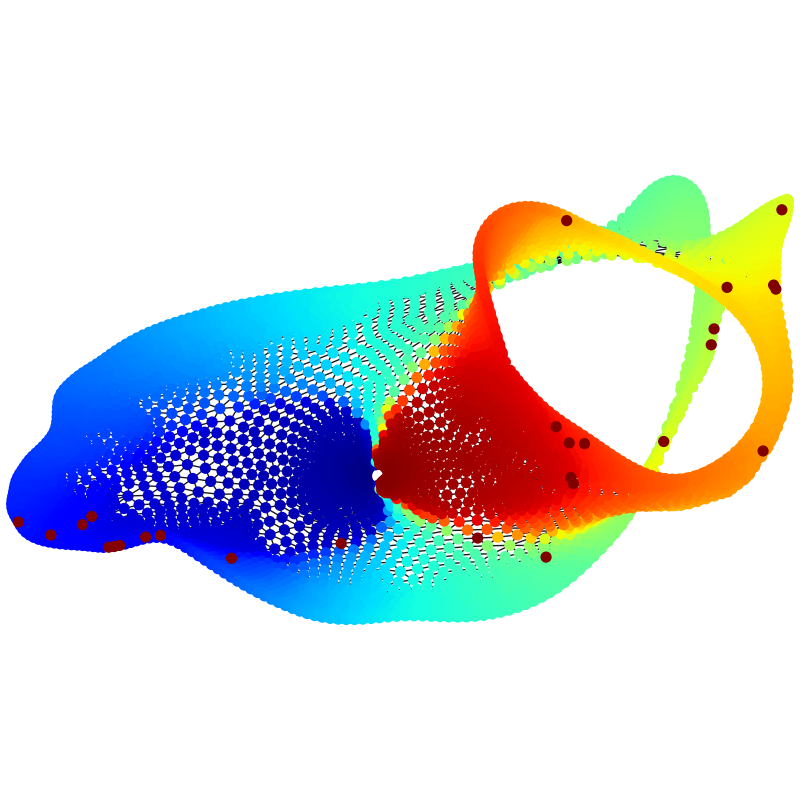
\includegraphics[width=0.135\columnwidth]{../main/individual/vis/opt_3elt.png}} \\
      \end{tabular}
      \caption{``BEST'' is the 500th iteration of the proposed algorithm.}
    \end{figure}
  \end{frame}
\fi

\ifShowHidden
  \begin{frame}{Experiments Result (overall)}
    As a dataset, we used matrices from Sparse Matrix Collection~\cite{davis2011university}, in total 124 graphs.
    \begin{figure}[h]
      \centering
      \begin{minipage}{0.5\columnwidth}
        \centering
        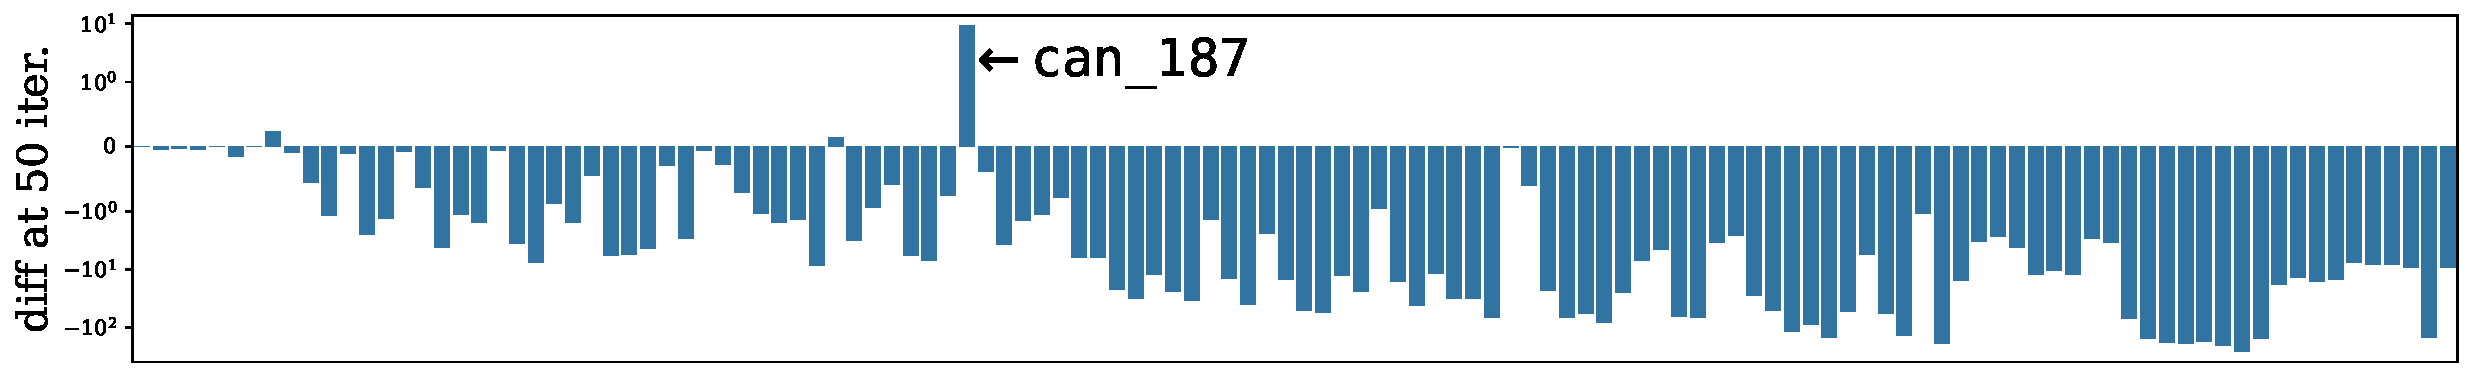
\includegraphics[width=\columnwidth]{../main/overall/plot/diff_FR_50.pdf}
      \end{minipage}%
      \begin{minipage}{0.5\columnwidth}
        \centering
        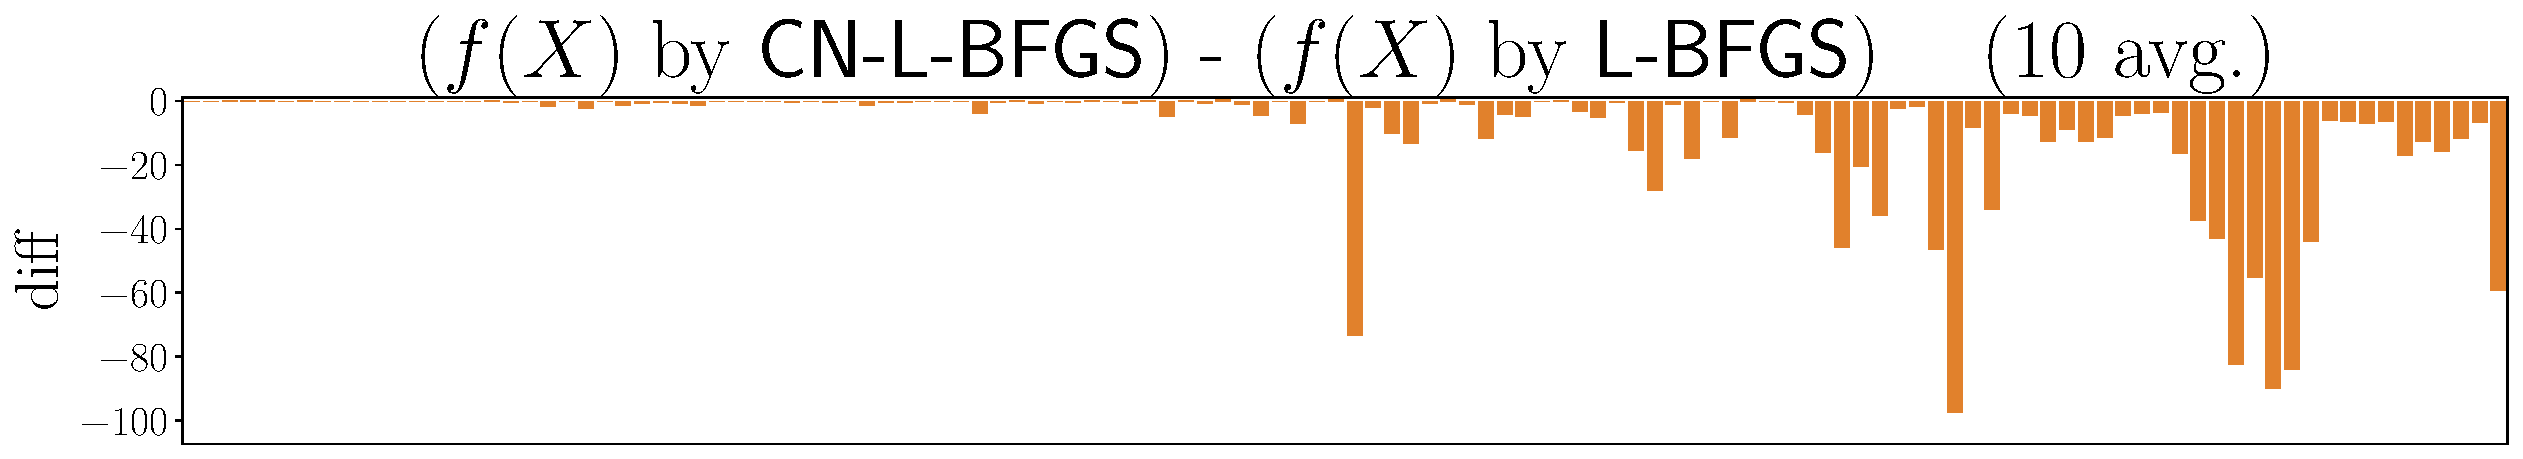
\includegraphics[width=\columnwidth]{../main/overall/plot/diff_L-BFGS_50.pdf}
      \end{minipage}%
      \caption{
        45th iter proposed initialization (\textsf{CN}) vs. 50th iter random initialization (no prefix).
      }
      \label{fig:overall}
    \end{figure}
    \begin{figure}[h]
      \centering
      \begin{minipage}{0.5\columnwidth}
        \centering
        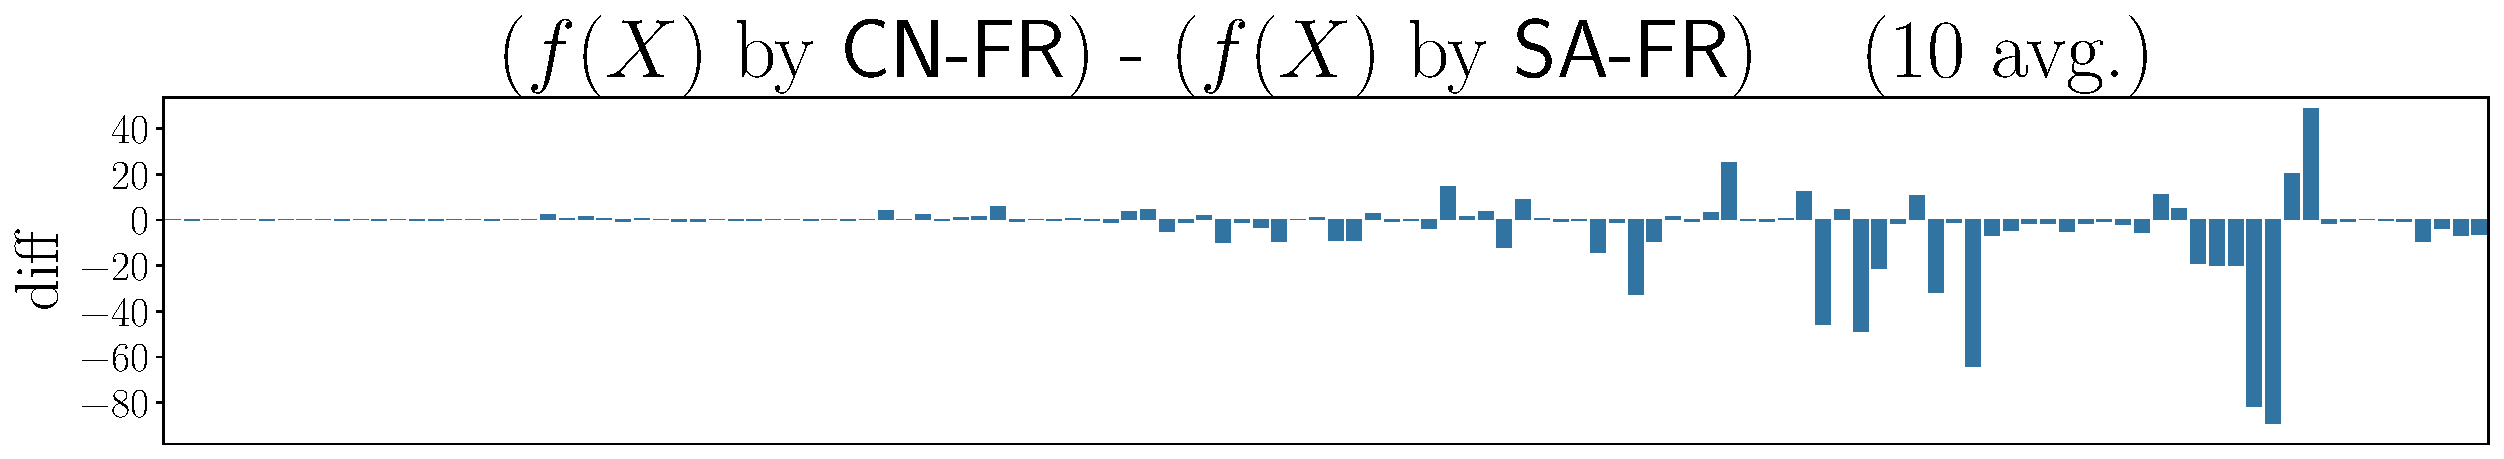
\includegraphics[width=\columnwidth]{../main/circle/plot/diff_FR_50.pdf}
      \end{minipage}%
      \begin{minipage}{0.5\columnwidth}
        \centering
        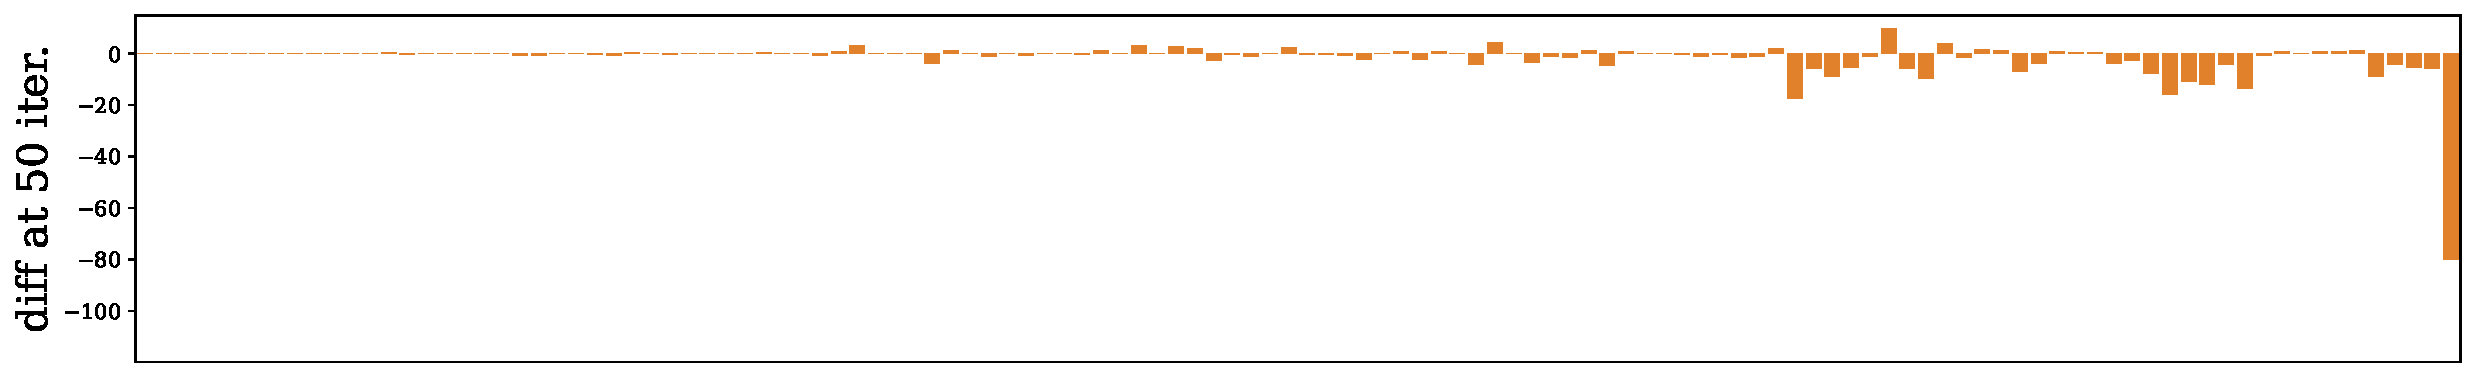
\includegraphics[width=\columnwidth]{../main/circle/plot/diff_L-BFGS_50.pdf}
      \end{minipage}%
      \caption{
        50th iter proposed initialization (\textsf{CN}) vs. 50th iter circle initialization (\textsf{SA})~\cite{ghassemitoosiSimulatedAnnealingPreProcessing2016}.
      }
      \label{fig:diff}
    \end{figure}
  \end{frame}
\fi

\ifShowHidden
  \begin{frame}{Comparision with SA method}
    \begin{figure}[t]
      \centering
      \begin{tabular}{cccccc}
        \toprule
         & \multicolumn{2}{c}{\texttt{dwt\_992} (\textsf{SA} better)}
         & \multicolumn{2}{c}{\texttt{collins\_15NN} (\textsf{CN} better)}                                                                                          \\
         & initial placement                                                                                & 50th iteration & initial placement & 50th iteration & \\
        \cmidrule(lr){2-3} \cmidrule(lr){4-5}
        \rotatebox{90}{\textsf{SA} (Ref.~\cite{ghassemitoosiSimulatedAnnealingPreProcessing2016})}
         & 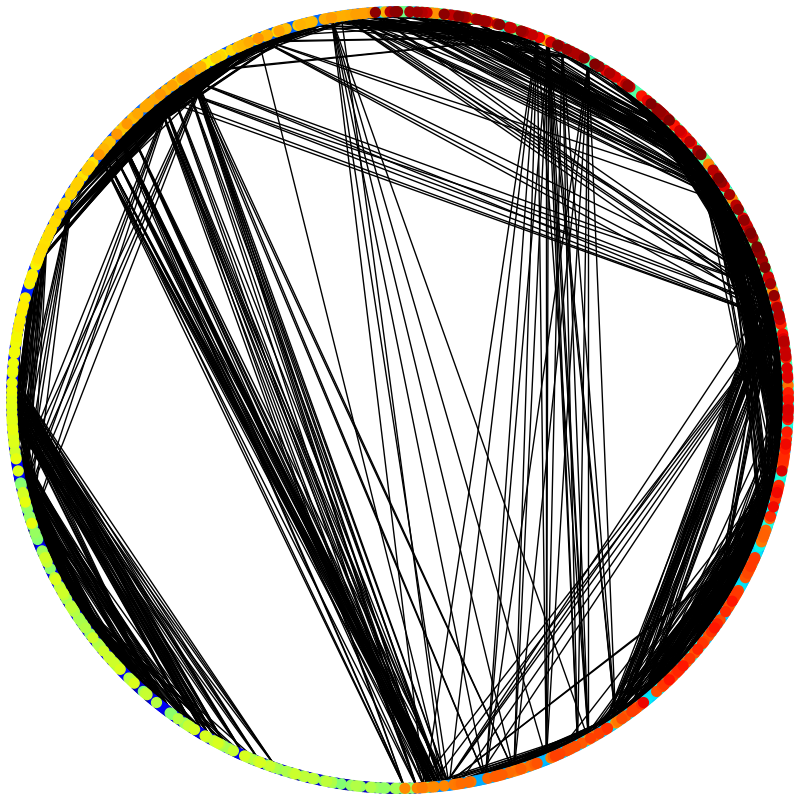
\includegraphics[width=0.15\columnwidth]{../main/circle/vis/dwt_992_SA-L-BFGS_50_first.png}
         & 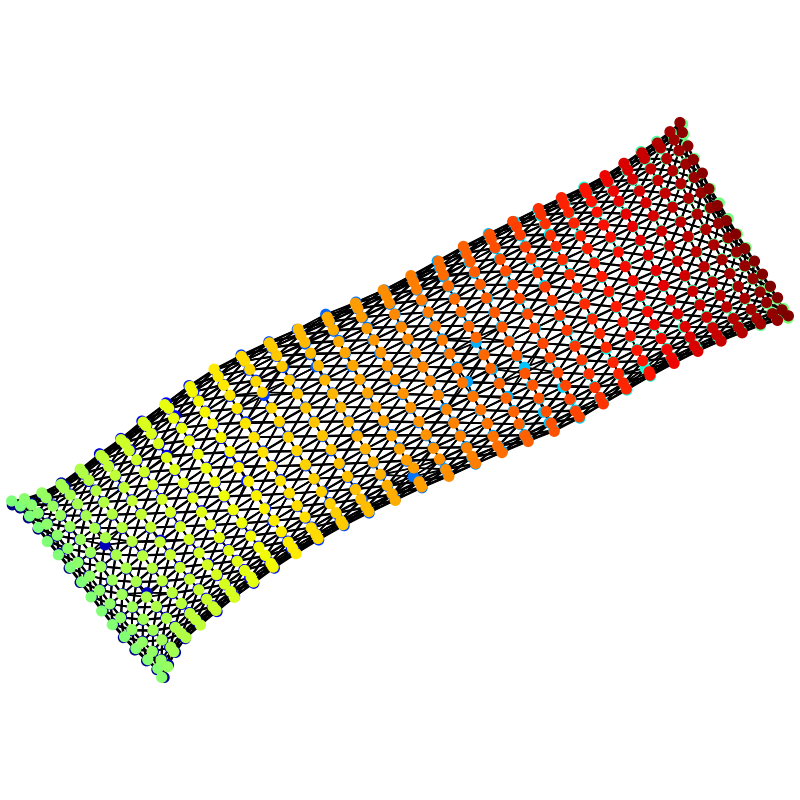
\includegraphics[width=0.15\columnwidth]{../main/circle/vis/dwt_992_SA-L-BFGS_50_last.png}
         & 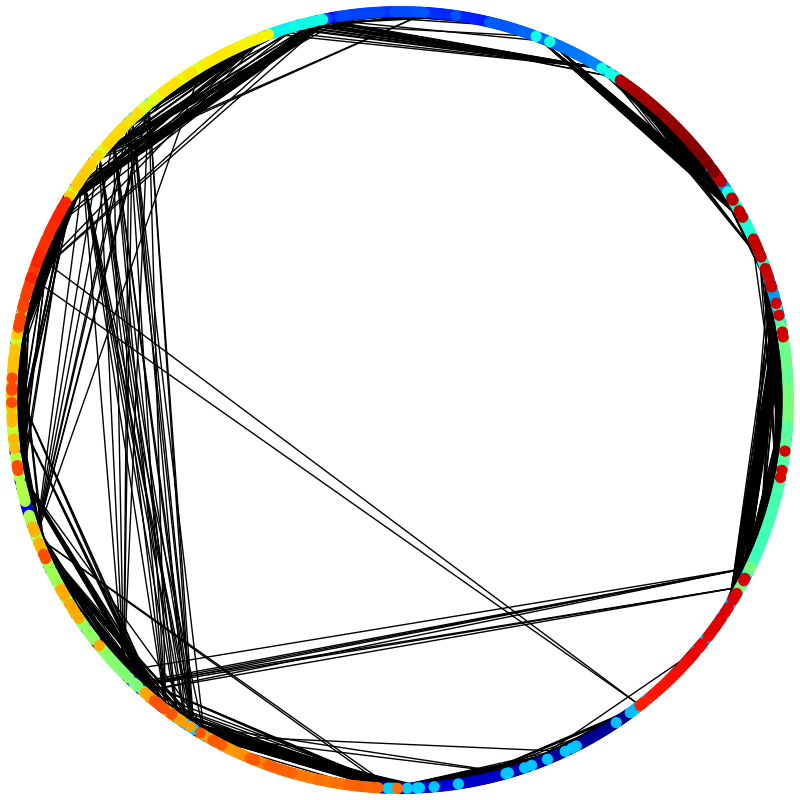
\includegraphics[width=0.15\columnwidth]{../main/circle/vis/collins_15NN_SA-L-BFGS_50_first.png}
         & \includegraphics[width=0.15\columnwidth]{../main/circle/vis/collins_15NN_SA-L-BFGS_50_last.png}                                                          \\
        \addlinespace
        \rotatebox{90}{\textsf{CN} (proposed)}
         & \includegraphics[width=0.15\columnwidth]{../main/circle/vis/dwt_992_CN-L-BFGS_50_first.png}
         & \includegraphics[width=0.15\columnwidth]{../main/circle/vis/dwt_992_CN-L-BFGS_50_last.png}
         & \includegraphics[width=0.15\columnwidth]{../main/circle/vis/collins_15NN_CN-L-BFGS_50_first.png}
         & \includegraphics[width=0.15\columnwidth]{../main/circle/vis/collins_15NN_CN-L-BFGS_50_last.png}                                                          \\
        \bottomrule
      \end{tabular}
      \caption{\small{Results showing initial and 50th iteration placements for \texttt{dwt\_992} and \texttt{collins\_15NN}.}}
      \label{fig:CN_vs_SA}
    \end{figure}
  \end{frame}
\fi

\section{Discussion}

% \ifShowHidden
%   \begin{frame}{Rationale of the Proposed Method}
%     \begin{columns}
%       \begin{column}{0.5\columnwidth}
%         \textbf{Q}: Why we cannot directly apply coordinate descent to the problem~\eqref{eq:fr}?\\
%         \textbf{A}: The ignorance of other vertices' movements.\\
%         \vspace{0.5cm}
%         Discrete optimization problem \\
%         $\to$ \textbf{At least $\epsilon$} movement\\
%         $\to$ \textbf{More efficient} than direct application.
%       \end{column}
%       \begin{column}{0.5\columnwidth}
%         \begin{figure}[h]
%           \centering
%           \includegraphics[width=\columnwidth]{../main/whyRSNfail2/whyRSNfail2.pdf}
%           \caption{
%             The ignorance of other vertex movements.
%             Although the blue arrows show the forces in this situation, the red vertex barely moves by the coordinate Newton direction.
%           }
%         \end{figure}
%       \end{column}
%     \end{columns}
%   \end{frame}
% \fi

\ifShowHidden
  \begin{frame}{Future Work (1/2) - Combine with \texttt{sfdp}}
    \begin{columns}
      \begin{column}{0.5\columnwidth}
        \textbf{\texttt{sfdp} in Graphviz \raisebox{-0.2\baselineskip}{\includegraphics[width=1.5em]{graphDrawing/GraphvizLogo.png}}~\cite{ellsonGraphvizOpenSource2002}}\\
        \quad \textbf{S}calable \textbf{F}orce-\textbf{D}irected \textbf{P}lacement.\\
        \quad This is a \textbf{Multilevel} approach.\\
        \quad Barnes--Hut algorithm (Q-tree)\cite{Hu2006EfficientHF,barnesHierarchicalLogForcecalculation1986}.\\
        \quad These methods are\\
        \quad compatible with the proposed method.
      \end{column}
      \begin{column}{0.5\columnwidth}
        \begin{figure}[htbp]
          \centering
          \includegraphics[width=0.7\columnwidth]{imgs/BH.png}
          \caption{\footnotesize{\href{https://jheer.github.io/barnes-hut/}{link}}}
        \end{figure}
      \end{column}
    \end{columns}
  \end{frame}
\fi

\ifShowHidden
  \begin{frame}{Future Work (2/2) - Broader Applications}
    \textbf{``objective functions arising from graphs''}~\cite{recht-wright}\\
    \begin{equation*}
      f(X) = \sum_{\{i,j\}\in E} f_{i,j}(x_i, x_j)
      +\lambda \sum_{i=1}^{n} \Omega_i(x_i)
    \end{equation*}
    General optimization problem arising from graphs.\\
    \textbf{stochastic coordinate descent}~\cite{recht-wright} only with \text{the gradient} is popular.\\
    Can we use coordinate Newton direction?
    \begin{columns}
      \begin{column}{0.5\columnwidth}
        \textbf{Graph Isomorphism Problem}\\
        Drawing graph symmetry is at least as difficult as the graph isomorphism problem~\cite{eades1984heuristic}.\\
        Continuous relaxation $\to$ optimization on Riemannian manifolds~\cite{klusContinuousOptimizationMethods2023}\\
        Can we utilize coordinate Newton direction for Riemannian optimization?\\
      \end{column}
      \begin{column}{0.5\columnwidth}
        \begin{figure}[t]
          \centering
          \includegraphics[width=\columnwidth]{../main/iso/iso.pdf}
        \end{figure}
      \end{column}
    \end{columns}
  \end{frame}
\fi

\ifShowHidden
  \begin{frame}{End of the Presentation}
    \begin{block}{Summary}
      \quad Fruchterman--Reingold layout is a tough problem\\
      \quad Hexagonal Lattice + coordinate Newton direction\\
      \quad initialization + L-BFGS gives the best result
    \end{block}
    \begin{block}{Acknowledgement}
      \large{
        I would like to express my sincere gratitude to \textbf{Pierre-Louis Poirion}, \textbf{Andi Han}, and \textbf{Naoki Marumo}.
      }
    \end{block}
  \end{frame}
\fi

\setbeamercolor{structure}{fg=blendedblue}
\setbeamercolor{block title}{fg=blendedblue!50!black}

\ifShowHidden
  \begin{frame}[allowframebreaks]{Reference}
    \scriptsize
    \beamertemplatetextbibitems
    \bibliographystyle{IEEEtran}
    \bibliography{../main/FruchtermanReingoldByRandomSubspace.bib}
    % \begin{thebibliography}{1}
    % \end{thebibliography}
  \end{frame}
\fi

\end{document}